%%%%%%%%%%%%%%%%%%%%%%%%%%%%%%% beamer %%%%%%%%%%%%%%%%%%%%%%%%%%%%%%%%%%%%%%%%%%%%%%%%%
% To run - pdflatex filename.tex
%      acroread filename.pdf
%%%%%%%%%%%%%%%%%%%%%%%%%%%%%%%%%%%%%%%%%%%%%%%%%%%%%%%%%%%%%%%%%%%%%%%%%%%%%%%%%%%%%%%%

\documentclass[compress,oilve]{beamer}
\mode<presentation>

\usetheme[]{CambridgeUS}
% other themes: AnnArbor, Antibes, Bergen, Berkeley, Berlin, Boadilla, boxes, CambridgeUS, Copenhagen, Darmstadt, default, Dresden, Frankfurt, Goettingen,
% Hannover, Ilmenau, JuanLesPins, Luebeck, Madrid, Maloe, Marburg, Montpellier, PaloAlto, Pittsburg, Rochester, Singapore, Szeged, classic

\usecolortheme{beaver}
% color themes: albatross, beaver, beetle, crane, default, dolphin,  fly, lily, orchid, rose, seagull, seahorse, sidebartab, whale, wolverine

\usefonttheme{professionalfonts}
% font themes: default, professionalfonts, serif, structurebold, structureitalicserif, structuresmallcapsserif


\hypersetup{pdfpagemode=FullScreen} % makes your presentation go automatically to full screen

% define your own colors:
\definecolor{Red}{rgb}{1,0,0}
\definecolor{Blue}{rgb}{0,0,1}
\definecolor{Green}{rgb}{0,1,0}
\definecolor{magenta}{rgb}{1,0,.6}
\definecolor{lightblue}{rgb}{0,.5,1}
\definecolor{lightpurple}{rgb}{0.8, 0.6, 0.9}
\definecolor{gold}{rgb}{.6,.5,0}
\definecolor{orange}{rgb}{1,0.4,0}
\definecolor{hotpink}{rgb}{1,0,0.5}
\definecolor{newcolor2}{rgb}{.5,.3,.5}
\definecolor{newcolor}{rgb}{0,.3,1}
\definecolor{newcolor3}{rgb}{1,0,.35}
\definecolor{darkgreen1}{rgb}{0, .35, 0}
\definecolor{darkgreen}{rgb}{0, .6, 0}
\definecolor{darkred}{rgb}{.75,0,0}
\definecolor{skyblue}{HTML}{75bbfd}

\definecolor{olive}{cmyk}{0.64,0,0.95,0.4}
\definecolor{purpleish}{cmyk}{0.75,0.75,0,0}


% % Define a custom color
% \definecolor{backcolour}{rgb}{0.95,0.95,0.92}
% \definecolor{codegreen}{rgb}{0,0.6,0}

% \usepackage{listings}

% % Define a custom style
% \lstdefinestyle{myStyle}{
%     backgroundcolor=\color{backcolour},   
%     commentstyle=\color{codegreen},
%     basicstyle=\ttfamily\tinytosmallsize,
%     breakatwhitespace=false,         
%     breaklines=true,                 
%     keepspaces=true,                 
%     numbers=left,       
%     numbersep=5pt,                  
%     showspaces=false,                
%     showstringspaces=false,
%     showtabs=false,                  
%     tabsize=2,
% }

% % Use \lstset to make myStyle the global default
% \lstset{style=myStyle}
% color def
\usepackage{color}
\definecolor{darkred}{rgb}{0.6,0.0,0.0}
\definecolor{darkgreen}{rgb}{0,0.50,0}
\definecolor{lightblue}{rgb}{0.0,0.42,0.91}
\definecolor{orange}{rgb}{0.99,0.48,0.13}
\definecolor{grass}{rgb}{0.18,0.80,0.18}
\definecolor{pink}{rgb}{0.97,0.15,0.45}

% listings
\usepackage{listings}

% General Setting of listings
\lstset{
  aboveskip=1em,
  breaklines=true,
  abovecaptionskip=5pt,
  captionpos=b,
  escapeinside={\%*}{*)},
  frame=single,
  numbers=left,
  numbersep=15pt,
  numberstyle=\tiny,
}
% 0. Basic Color Theme
\lstdefinestyle{colored}{ %
  basicstyle=\ttfamily,
  backgroundcolor=\color{white},
  commentstyle=\color{green}\itshape,
  keywordstyle=\color{blue}\bfseries\itshape,
  stringstyle=\color{red},
}
% 1. General Python Keywords List
\lstdefinelanguage{PythonPlus}[]{Python}{
  morekeywords=[1]{,as,assert,nonlocal,with,yield,self,True,False,None,} % Python builtin
  morekeywords=[2]{,__init__,__add__,__mul__,__div__,__sub__,__call__,__getitem__,__setitem__,__eq__,__ne__,__nonzero__,__rmul__,__radd__,__repr__,__str__,__get__,__truediv__,__pow__,__name__,__future__,__all__,}, % magic methods
  morekeywords=[3]{,object,type,isinstance,copy,deepcopy,zip,enumerate,reversed,list,set,len,dict,tuple,range,xrange,append,execfile,real,imag,reduce,str,repr,}, % common functions
  morekeywords=[4]{,Exception,NameError,IndexError,SyntaxError,TypeError,ValueError,OverflowError,ZeroDivisionError,}, % errors
  morekeywords=[5]{,ode,fsolve,sqrt,exp,sin,cos,arctan,arctan2,arccos,pi, array,norm,solve,dot,arange,isscalar,max,sum,flatten,shape,reshape,find,any,all,abs,plot,linspace,legend,quad,polyval,polyfit,hstack,concatenate,vstack,column_stack,empty,zeros,ones,rand,vander,grid,pcolor,eig,eigs,eigvals,svd,qr,tan,det,logspace,roll,min,mean,cumsum,cumprod,diff,vectorize,lstsq,cla,eye,xlabel,ylabel,squeeze,}, % numpy / math
}
% 2. New Language based on Python
\lstdefinelanguage{PyBrIM}[]{PythonPlus}{
  emph={d,E,a,Fc28,Fy,Fu,D,des,supplier,Material,Rectangle,PyElmt},
}
% 3. Extended theme
\lstdefinestyle{colorEX}{
  basicstyle=\ttfamily,
  backgroundcolor=\color{white},
  commentstyle=\color{darkgreen}\slshape,
  keywordstyle=\color{blue}\bfseries\itshape,
  keywordstyle=[2]\color{blue}\bfseries,
  keywordstyle=[3]\color{grass},
  keywordstyle=[4]\color{red},
  keywordstyle=[5]\color{orange},
  stringstyle=\color{darkred},
  emphstyle=\color{pink}\underbar,
}
\lstset{style=colored}

% can also choose different themes for the "inside" and "outside"

% \usepackage{beamerinnertheme_______}
% inner themes include circles, default, inmargin, rectangles, rounded

% \usepackage{beamerouterthemesmoothbars}
% outer themes include default, infolines, miniframes, shadow, sidebar, smoothbars, smoothtree, split, tree


\useoutertheme[subsection=true, height=40pt]{smoothbars}

% to have the same footer on all slides
%\setbeamertemplate{footline}[text line]{STUFF HERE!}
\setbeamertemplate{footline}[text line]{} % makes the footer EMPTY
% include packages
%

%show the page numbers in footnote
%\addtobeamertemplate{navigation symbols}{}{%
%	\usebeamerfont{footline}%
%	\usebeamercolor[fg]{footline}%
%	\hspace{1em}%
%	\insertframenumber/\inserttotalframenumber
%}

\setbeamercolor{footline}{fg=purpleish}
\setbeamerfont{footline}{series=\bfseries}

%add color to curent subsection
\setbeamertemplate{section in head/foot}{\hfill\tikz\node[rectangle, fill=darkred, rounded corners=1pt,inner sep=1pt,] {\textcolor{white}{\insertsectionhead}};}
\setbeamertemplate{section in head/foot shaded}{\textcolor{darkred}{\hfill\insertsectionhead}}

% Remove bullet of subsections
\setbeamertemplate{headline}
{%
	\begin{beamercolorbox}{section in head/foot}
		\insertsectionnavigationhorizontal{\textwidth}{}{}
	\end{beamercolorbox}%
}


% modify headlline, specially headline size
\setbeamertemplate{headline}{%
	\leavevmode%
	\hbox{%
		\begin{beamercolorbox}[wd=\paperwidth,ht=3.5ex,dp=1.125ex]{palette quaternary}%
			\insertsectionnavigationhorizontal{\paperwidth}{}{\hskip0pt plus1filll}
		\end{beamercolorbox}%
	}
}

\setbeamertemplate{footline}{%
	\leavevmode%
	\hbox{\begin{beamercolorbox}[wd=.5\paperwidth,ht=2.5ex,dp=1.125ex,leftskip=.3cm plus1fill,rightskip=.3cm]{author in head/foot}%
			\usebeamerfont{author in head/foot}\insertshortauthor ~ \insertshortinstitute
		\end{beamercolorbox}%
		\begin{beamercolorbox}[wd=.5\paperwidth,ht=2.5ex,dp=1.125ex,leftskip=.3cm,rightskip=.3cm plus1fil]{title in head/foot}%
			\usebeamerfont{title in head/foot}\insertshorttitle\hfill\insertframenumber\,/\,\inserttotalframenumber
	\end{beamercolorbox}}%
	\vskip0pt%
}


%\setbeamertemplate{navigation symbols}{}

\title{Autoencoders}
\author{ML Instruction Team, Fall 2022}
\institute[]{CE Department \newline  Sharif University of Technology \newline \newline \newline
            Mahsa Yazdani\newline
            Arian Amani}
\date[\today]{}
%\titlegraphic{\includegraphics[scale=.35]{example-image}}



%Write \usepackage{etex} just after the \documentclass line (it should be the first loaded package).
\usepackage{etex}
\usepackage{subcaption}
\usepackage{caption}
\usepackage{multicol}
\usepackage{amsmath}
\usepackage{epsfig}
\usepackage{graphicx}
\usepackage[all,knot]{xy}
\xyoption{arc}
\usepackage{url}
\usepackage{multimedia}
\usepackage{hyperref}
\hypersetup{colorlinks,linkcolor=blue,citecolor=red,urlcolor=darkred}
\usepackage{multirow}
\usepackage[font={scriptsize}]{caption}
\usepackage{pgf}
\usepackage{fontspec}
\usepackage{svg}

% \usepackage{biblatex}
% \addbibresource{Refrences.bib}
% \AtBeginBibliography{\small}


%\setsansfont[Scale=MatchLowercase, BoldFont = * Bold, ItalicFont = * Italic]{Caladea}

%\usepackage{enumitem,xcolor}
%\newcommand{\labelitemi}{$\blacksquare$}
%\newcommand{\labelitemii}{$\diamond$}
%\newcommand{\labelitemiii}{$\square$}
%\newcommand{\labelitemiv}{$\ast$}
%\setbeamercolor*{item}{fg=red}

% abbreviation
% \newrobustcmd{\B}{\bfseries}

\usefonttheme{professionalfonts} 
\setbeamertemplate{itemize item}{\color{skyblue}$\blacksquare$}
\setbeamertemplate{itemize subitem}{\color{hotpink}$\blacktriangleright$}
\setbeamertemplate{itemize subsubitem}{\color{orange}$\bullet$}


\usepackage{anyfontsize}
\usepackage{t1enc}
\usepackage{tikz}
\usetikzlibrary{calc,trees,positioning,arrows,chains,shapes.geometric,decorations.pathreplacing,decorations.pathmorphing,shapes,matrix,shapes.symbols}



\newtheorem{proposition}[theorem]{Proposition}
\newtheorem{remark}[theorem]{Remark}
\newtheorem{assumption}[theorem]{Assumption}

\usepackage{xcolor}
\newcommand{\tc}[2]{
	\textcolor{#1}{#2}
}

%\usepackage{fontspec, unicode-math}
%\setmainfont[Scale=0.9]{Nimbus Roman No9 L}
%\setmonofont[Scale=0.9]{Monaco}
\setsansfont[Scale=1]{Times New Roman}

\newcommand{\vect}[1]{\boldsymbol{#1}}

\definecolor{strings}{rgb}{.624,.251,.259}
\definecolor{keywords}{rgb}{.224,.451,.686}
\definecolor{comment}{rgb}{.322,.451,.322}


%\usepackage{smartdiagram}
%\usesmartdiagramlibrary{additions}
%%%%%%%%%%%%%%%%%%%%%%%%%%%%%%%%%%%%%%%%%%%%%%%%%%%%%%%%%%%%%%%%%%%%%%%%%%%%%%%%%%%%%%%%%%%%
%%%%%%%%%%%%%%%%%%%%%%%%%%%%%% Title Page Info %%%%%%%%%%%%%%%%%%%%%%%%%%%%%%%%%%%%%%%%%%%
%%%%%%%%%%%%%%%%%%%%%%%%%%%%%%%%%%%%%%%%%%%%%%%%%%%%%%%%%%%%%%%%%%%%%%%%%%%%%%%%%%%%%%%%%%


%%%%%%%%%%%%%%%%%%%%%%%%%%%%%%%%%%%%%%%%%%%%%%%%%%%%%%%%%%%%%%%%%%%%%%%%%%%%%%%%%%%%%%%%%%
%%%%%%%%%%%%%%%%%%%%%%%%%%%%%% Begin Your Document %%%%%%%%%%%%%%%%%%%%%%%%%%%%%%%%%%%%%%%
%%%%%%%%%%%%%%%%%%%%%%%%%%%%%%%%%%%%%%%%%%%%%%%%%%%%%%%%%%%%%%%%%%%%%%%%%%%%%%%%%%%%%%%%%%
\begin{document}
	
%%%%%%%%%%%%%%%%%%%%%%%%%%%%%%%%%%%%%%%%%%%%%%%%%%%%%%%%%%%%%%%%%%%%%%%%%%%%%%%%%%%%%%%%%%
	\fontsize{9}{9}
\begin{frame}[noframenumbering, plain]
	\titlepage
\end{frame}

%%%%%%%%%%%%%%%%%%%%%%%%%%%%%%%%%%%%%%%%%%%%%%%%%%%%%%%%%%%%%%%%%%%%%%%%%%%%%%%%%%%%%%%%%%
\section{Introduction}
%%%%%%%%%%%%%%%%%%%%%%%%%%%%%%%%%%%%%%%%%%%%%%%%%%%%%%%%%%%%%%%%%%%%%%%%%%%%%%%%%%%%%%%%%%%%%%%

\frame{\frametitle{Let's Think}
	\centering
    % \vspace{25 pt}
    \textbf{\large{Let's start with a question!}}

}
%%%%%%%%%%%%%%%%%%%%%%%%%%%%%%%%%%%%%%%%%%%%%%%%%%%%%%%%%%%%%%%%%%%%%%%%%%%%%%%%%%%%%%%%%%%%%%%

\frame{\frametitle{Any ideas?}
    \begin{center}
    % \vspace{25 pt}
    \textbf{\large{How can we combine\tc{keywords}{neural networks}and\tc{keywords}{unlabeled data}to perform\tc{keywords}{compression}?}}
    \end{center}

    

}
%%%%%%%%%%%%%%%%%%%%%%%%%%%%%%%%%%%%%%%%%%%%%%%%%%%%%%%%%%%%%%%%%%%%%%%%######

\frame{\frametitle{The Power Of Unsupervised Learning}
\centering
\begin{itemize}
    \normalsize {
	\item Huge datasets compared to supervised learning (No need for labeling)
	\item Can find previously unknown patterns in data that are impossible with supervised learning
	}
\end{itemize}	
\begin{figure}
    \centering
    % \hspace{3cm}
    \captionsetup{justification=centering}
    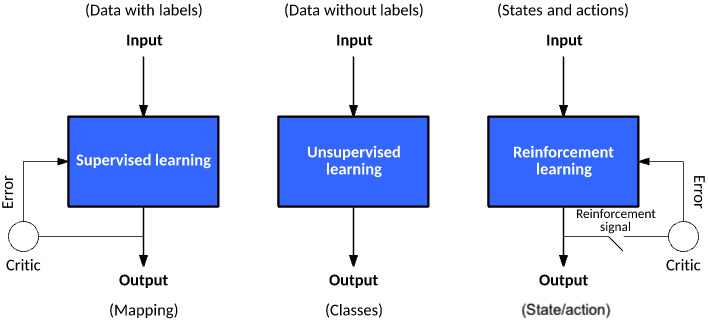
\includegraphics[width=11cm]{figs/unsupervised-learning.jpg}
    \caption{Types of Machine learning: Deep learning (supervised and\tc{keywords}{unsupervised learning})(Jones [2017]), \href{https://www.researchgate.net/figure/Types-of-Machine-learning-Deep-learning-supervised-and-unsupervised-learning-and_fig5_335569456}{Source}}
\end{figure}
}

%%%%%%%%%%%%%%%%%%%%%%%%%%%%%%%%%%%%%%%%%%%%%%%%%%%%%%%%%%%%%%%%%%%%%%%%######

\frame{\frametitle{Applications of Autoencoders}
\centering
\vspace{-0.2cm}
\begin{itemize}
    \normalsize {
	\item Compression:
	    \begin{itemize}
	        \item AEs can compress our input into a lower dimensional vector and try to reconstruct the original input from that vector
	    \end{itemize}
	}
\end{itemize}	
\begin{figure}
    \centering
    % \vspace{-1cm}
    \captionsetup{justification=centering, margin=1cm, labelformat=empty}
    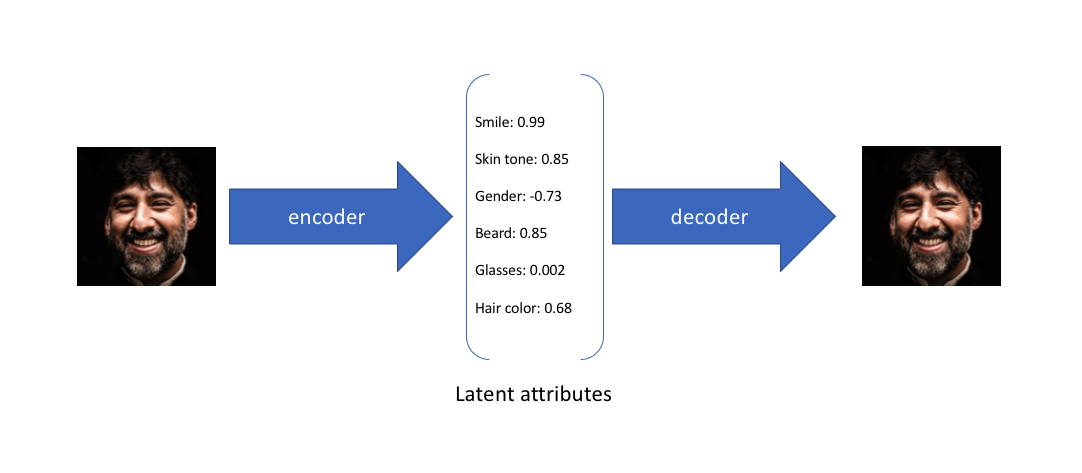
\includegraphics[width=12cm, height=5cm]{figs/Applications1.png}
    \caption{\href{https://www.jeremyjordan.me/variational-autoencoders/}{Source}}
\end{figure}
}

%%%%%%%%%%%%%%%%%%%%%%%%%%%%%%%%%%%%%%%%%%%%%%%%%%%%%%%%%%%%%%%%%%%%%%%%######

\frame{\frametitle{Applications of Autoencoders}
\centering
\vspace{-0.2cm}
\begin{itemize}
    \normalsize {
	\item Dimensionality Reduction:
	    \begin{itemize}
	        \item AEs can perform dimensionality reduction
	    \end{itemize}
	}
\end{itemize}	
\begin{figure}
    \centering
    % \vspace{-1cm}
    \captionsetup{justification=centering, margin=1cm, labelformat=empty}
    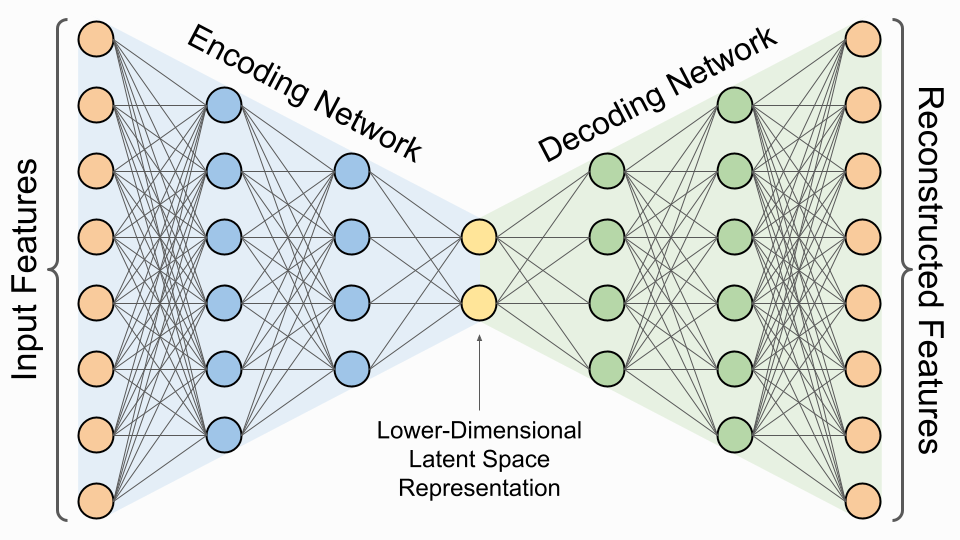
\includegraphics[width=12cm, height=5cm]{figs/Applications2.png}
    \caption{\href{https://www.assemblyai.com/blog/introduction-to-variational-autoencoders-using-keras/}{Source}}
\end{figure}
}

%%%%%%%%%%%%%%%%%%%%%%%%%%%%%%%%%%%%%%%%%%%%%%%%%%%%%%%%%%%%%%%%%%%%%%%%######

\frame{\frametitle{Applications of Autoencoders}
\centering
\vspace{-0.2cm}
\begin{itemize}
    \normalsize {
	\item Image coloring and noise reduction
	}
\end{itemize}	
\begin{figure}
    \centering
    % \vspace{-1cm}
    \captionsetup{justification=centering, margin=1cm, labelformat=empty}
    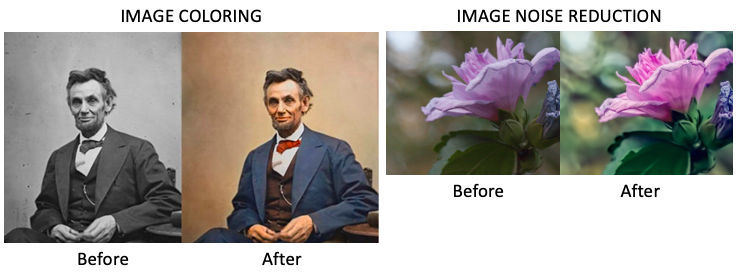
\includegraphics[width=12cm, height=5cm]{figs/Applications3.png}
    \caption{\href{https://towardsdatascience.com/convolutional-autoencoders-for-image-noise-reduction-32fce9fc1763}{Source}}
\end{figure}
}

%%%%%%%%%%%%%%%%%%%%%%%%%%%%%%%%%%%%%%%%%%%%%%%%%%%%%%%%%%%%%%%%%%%%%%%%######

\frame{\frametitle{Applications of Autoencoders}
\centering
\vspace{-0.2cm}
\begin{itemize}
    \normalsize {
	\item Noise reduction
	}
\end{itemize}	
\begin{figure}
    \centering
    % \vspace{-1cm}
    \captionsetup{justification=centering, margin=1cm, labelformat=empty}
    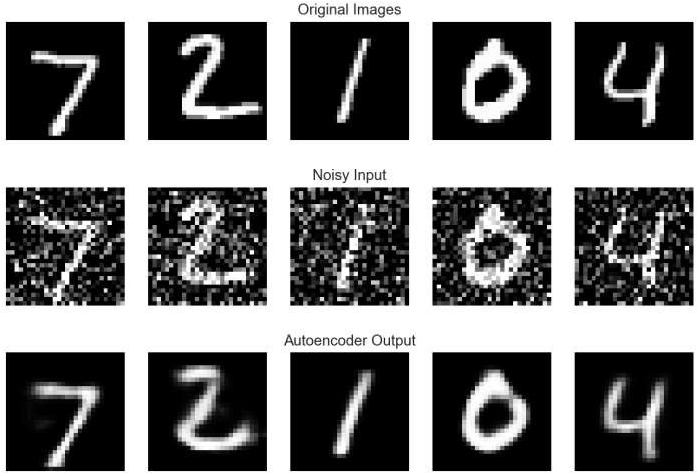
\includegraphics[width=12cm, height=5cm]{figs/noise_reduction.png}
    \caption{\href{https://towardsdatascience.com/applied-deep-learning-part-3-autoencoders-1c083af4d798}{Source}}
\end{figure}
}

%%%%%%%%%%%%%%%%%%%%%%%%%%%%%%%%%%%%%%%%%%%%%%%%%%%%%%%%%%%%%%%%%%%%%%%%######

\frame{\frametitle{Applications of Autoencoders}
\centering
\vspace{-0.2cm}
\begin{itemize}
    \normalsize {
	\item Watermark removal
	}
\end{itemize}	
\begin{figure}
    \centering
    % \vspace{-1cm}
    \captionsetup{justification=centering, margin=1cm, labelformat=empty}
    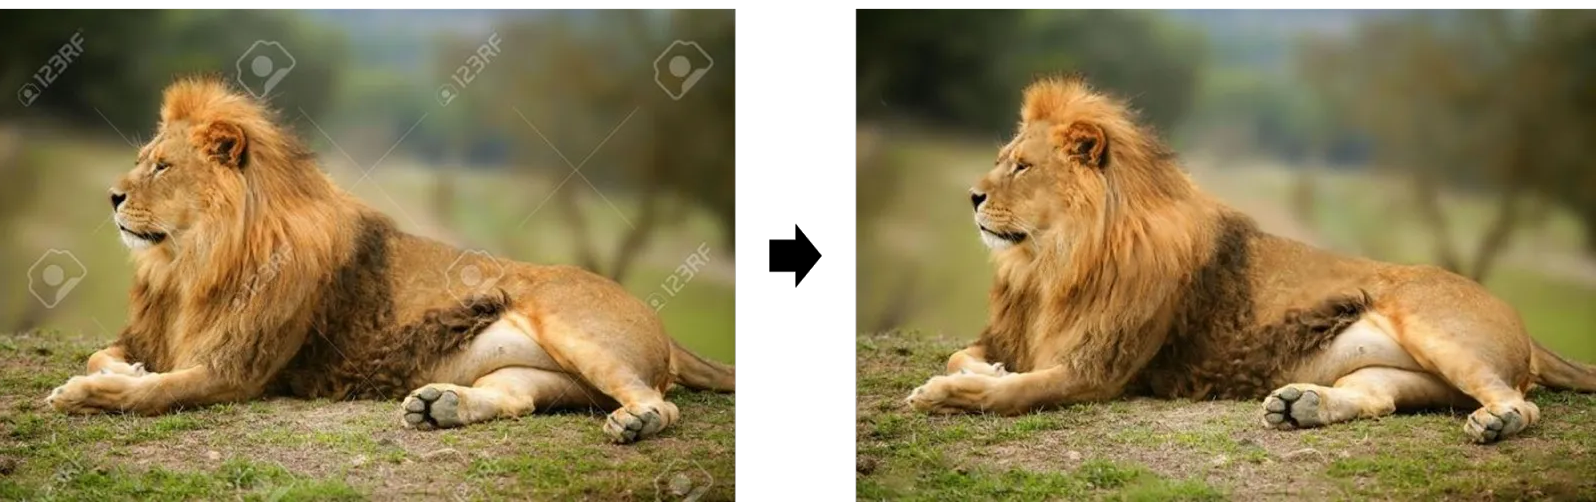
\includegraphics[width=12cm, height=5cm]{figs/watermark_removal.png}
    \caption{\href{https://watermark-cvpr17.github.io/}{Source}}
\end{figure}
}

%%%%%%%%%%%%%%%%%%%%%%%%%%%%%%%%%%%%%%%%%%%%%%%%%%%%%%%%%%%%%%%%%%%%%%%%######

\frame{\frametitle{Applications of Autoencoders}
% \centering
\vspace{-0.6cm}
\begin{itemize}
    \normalsize {
	\item Super-Resolution
	}
\end{itemize}	
\begin{figure}
    \centering
    \captionsetup{justification=centering, margin=1cm, labelformat=empty}
    \vspace{-0.4cm}
    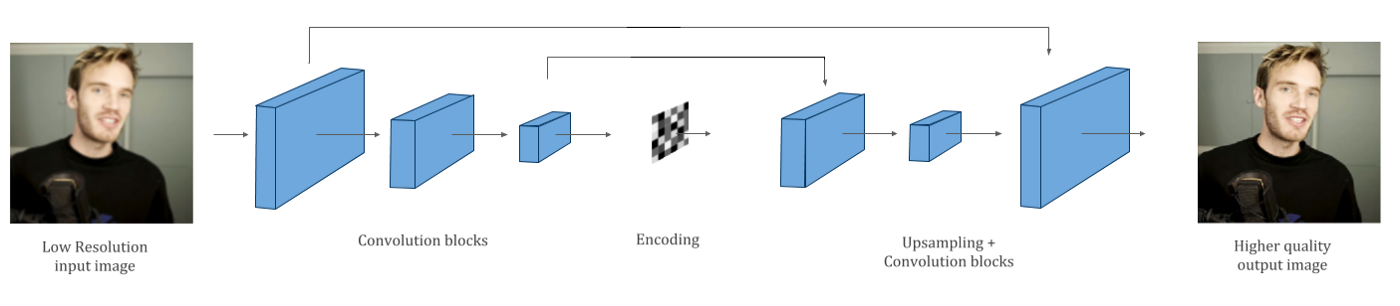
\includegraphics[width=11cm, height=5cm]{figs/Applications4.png}
    \caption{\href{https://towardsdatascience.com/improving-pewdiepies-camera-quality-with-autoencoders-583635de1cde}{Source}}
\end{figure}
}
%%%%%%%%%%%%%%%%%%%%%%%%%%%%%%%%%%%%%%%%%%%%%%%%%%%%%%%%%%%%%%%%%%%%%%%%%%%%%%%%%%%%%%%%%%
\section{Definition}
%%%%%%%%%%%%%%%%%%%%%%%%%%%%%%%%%%%%%%%%%%%%%%%%%%%%%%%%%%%%%%%%%%%%%%%%%%%%%%%%%%%%%%%%%%%%%%%

\frame{\frametitle{What is an Autoencoder?}
\vspace{-0.2cm}	

\begin{itemize}
    \normalsize{
	\item 
    An \tc{keywords}{autoencoder} is a type of artificial neural network, capable of learning a low dimensional representation of the input data (codings), without supervision (unlabeled training data - unsupervised learning)
	\item 
	Autoencoders take an input $X$ and try to predict $X$. We use a \tc{keywords}{bottleneck} layer with a smaller dimension compared to the input, to use as the coding.
    }
\end{itemize}	
\begin{figure}
    \centering
    % \captionsetup{justification=centering, margin=1cm, labelformat=empty}
    \captionsetup{justification=centering}
    \vspace{-0.22cm}
    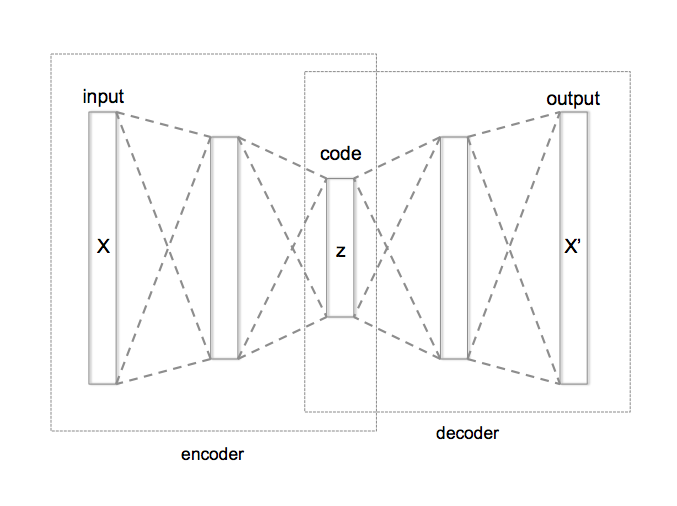
\includegraphics[width=10cm, height=4cm]{figs/Autoencoder1.png}
    \caption{Schematic structure of an autoencoder with 3 fully connected hidden layers. The code (z -\tc{keywords}{bottleneck}) is the most internal layer, \href{https://en.wikipedia.org/wiki/Autoencoder}{Source}}
\end{figure}

	
}

%%%%%%%%%%%%%%%%%%%%%%%%%%%%%%%%%%%%%%%%%%%%%%%%%%%%%%%%%%%%%%%%%%%%%%%%%%%%%%%%%%%%%%%%%%%%%%%
\frame{\frametitle{Autoencoders: Architecture}
\vspace{-0.1cm}	

\begin{itemize}
    \large{
    \item Autoencoders consist of 3 parts:
    % \vspace{0.2cm}
    \begin{enumerate}
        \normalsize{
        \item \tc{keywords}{Encoder}: \small Function $f(x)$ that transforms input $x$ to the latent variable $z$

        \item \tc{keywords}{Bottleneck}: \small Single layer of neurons that represent the encoding of our input, therefore the most important part of our model

        \item {\tc{keywords}{Decoder}: \small Function $h(z)$ that tries to reconstruct input $x$ from encoded latent variable $z$ {\rightarrow} \(h(z) = h(f(x)) = x'\)}
        }
    \end{enumerate}
    }
\end{itemize}

\begin{figure}
    \centering
    \vspace{-0.2cm}
    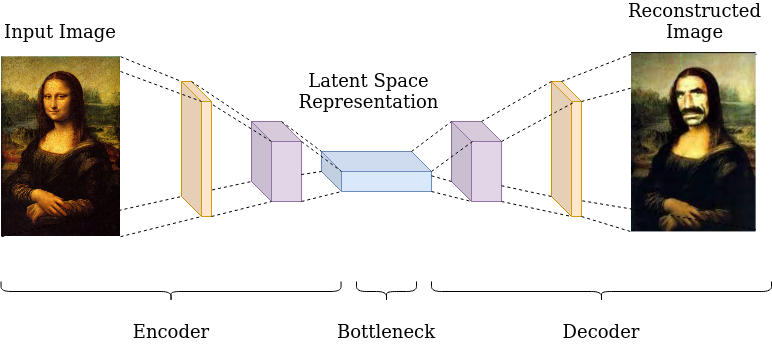
\includegraphics[width=10cm, height=4cm]{figs/Bad_AE.png}
    \caption{Autoencoder Architecture (with a little joke :)), \href{https://emkademy.medium.com/1-first-step-to-generative-deep-learning-with-autoencoders-22bd41e56d18}{Source}}
\end{figure}
}

%%%%%%%%%%%%%%%%%%%%%%%%%%%%%%%%%%%%%%%%%%%%%%%%%%%%%%%%%%%%%%%%%%%%%%%%%%%%%%%%%%%%%%%%%%%%%%%

\frame{\frametitle{Linear vs. Non-Linear}
\vspace{-1.3cm}
\begin{itemize}
    \normalsize{
	\item If your AE uses only linear activations and MSE loss function:
	    \begin{itemize}
	        \item It will be performing PCA (Principal Component Analysis)
	        \item So we need non-linearity to get the most out of autoencoders
	    \end{itemize}
	}
	\end{itemize}
	\lstinputlisting[language=Python]{codes/pca.py}

}
%%%%%%%%%%%%%%%%%%%%%%%%%%%%%%%%%%%%%%%%%%%%%%%%%%%%%%%%%%%%%%%%%%%%%%%%%%%%%%%%%%%%%%%%%%%%%%%

\frame{\frametitle{Linear vs. Non-Linear}
% \vspace{-1.5cm}
\begin{figure}
    \centering
    \captionsetup{justification=centering, margin=1cm, labelformat=empty}
    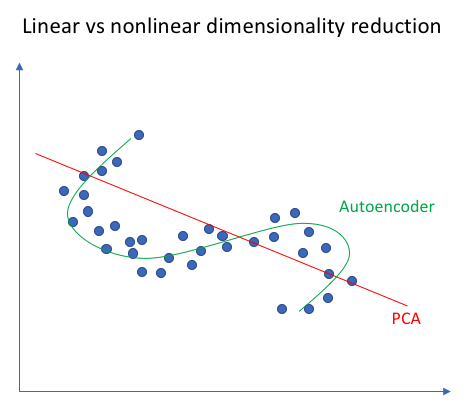
\includegraphics[width=8cm]{figs/AE_PCA.png}
    \caption{\href{https://www.jeremyjordan.me/autoencoders/}{Source}}
\end{figure}
}

%%%%%%%%%%%%%%%%%%%%%%%%%%%%%%%%%%%%%%%%%%%%%%%%%%%%%%%%%%%%%%%%%%%%%%%%%%%%%%%%%%%%%%%%%%%%%%%
\section{Stacked AE}
%%%%%%%%%%%%%%%%%%%%%%%%%%%%%%%%%%%%%%%%%%%%%%%%%%%%%%%%%%%%%%%%%%%%%%%%%%%%%%%%%%%%%%%%%%%%%%%

\frame{\frametitle{Stacked Autoencoders}
	
\begin{itemize}
    \normalsize{
	\item 
	Autoencoders can have multiple hidden layers to learn more complex encoding/decoding functions - \tc{keywords}{deep autoencoders}
	\vspace{0.1cm}
	\item
	Although, using too deep networks, can cause \tc{keywords}{overfitting}
	\vspace{0.1cm}
	    \begin{itemize}
	        \item
	        Your model will just memorize points in the coding space for each training data, instead of learning a good latent representation of them
	    \end{itemize}
	}
\end{itemize}	
\begin{figure}
    \centering
    % \vspace{-1cm}
    \captionsetup{justification=centering, margin=1cm, labelformat=empty}
    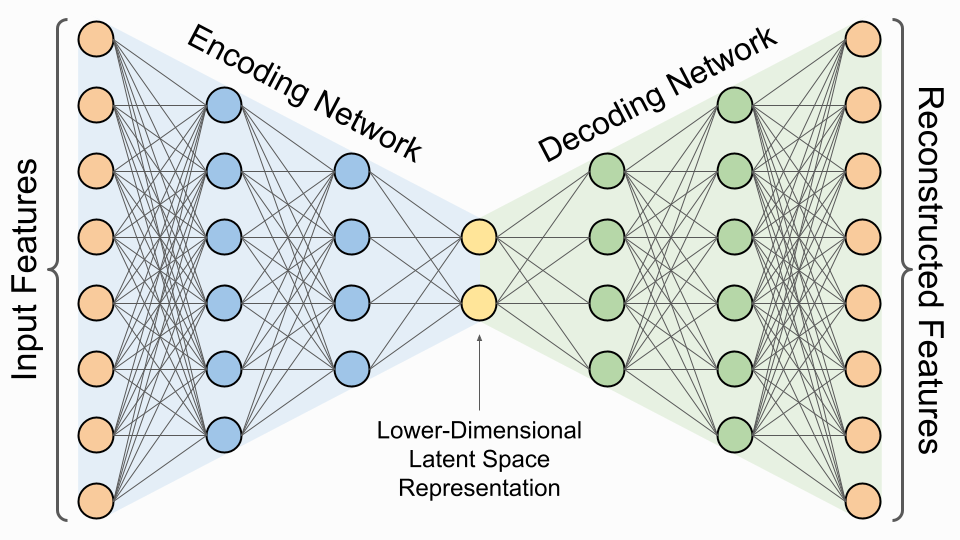
\includegraphics[width=12cm, height=4.3cm]{figs/Applications2.png}
    \caption{\href{https://www.assemblyai.com/blog/introduction-to-variational-autoencoders-using-keras/}{Source}}
\end{figure}
}

%%%%%%%%%%%%%%%%%%%%%%%%%%%%%%%%%%%%%%%%%%%%%%%%%%%%%%%%%%%%%%%%%%%%%%%%%%%%%%%%%%%%%%%%%%%%%%%

\frame{\frametitle{Loss and Training}
% \vspace{-3cm}
\begin{itemize}
    \normalsize{
	\item 
	We're trying to reconstruct our input
	\vspace{0.1cm}
	\item
	Common loss functions for training autoencoders are:
	\vspace{0.1cm}
	\begin{itemize}
	    \item{L2: $loss(x, x') = \sum^{m}_{i=1}(x^{(i)} - x'^{(i)})^2$}
    	\vspace{0.05cm}
	    \item{Cross-Entropy}
	\end{itemize}
	}
\end{itemize}

\begin{figure}
    \centering
    \vspace{-0.3cm}
    \captionsetup{justification=centering}
    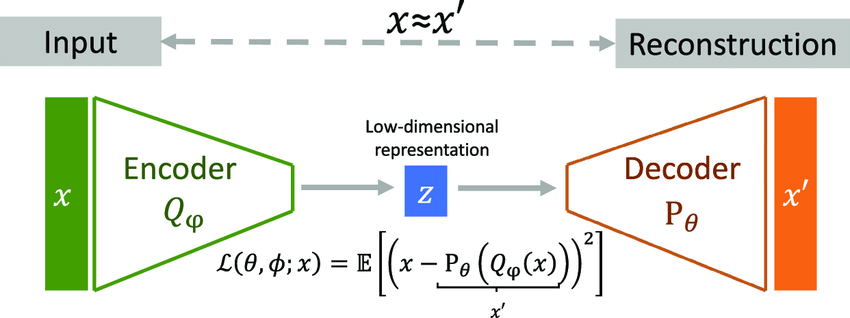
\includegraphics[width=10cm]{figs/AE_MSE.png}
    \caption{Schematic of an autoencoder architecture with mean-squared error reconstruction loss.\cite{MSE_AE}}
\end{figure}
}


%%%%%%%%%%%%%%%%%%%%%%%%%%%%%%%%%%%%%%%%%%%%%%%%%%%%%%%%%%%%%%%%%%%%%%%%%%%%%%%%%%%%%%%%%%%%%%%

\frame{\frametitle{Pretraining}
% \vspace{-3cm}
\begin{itemize}
    \normalsize{
	\item 
	You can use an autoencoder for pretraining on supervised problems with few labeled data
    }
\end{itemize}

\begin{figure}
    \centering
    \vspace{-4.5cm}
    \captionsetup{justification=centering}
    \includesvg[width=13cm, height=9cm]{figs/pretrain.svg}
    \caption{Using unsupervised learning for pretraining with autoencoders}
\end{figure}
}

%%%%%%%%%%%%%%%%%%%%%%%%%%%%%%%%%%%%%%%%%%%%%%%%%%%%%%%%%%%%%%%%%%%%%%%%%%%%%%%%%%%%%%%%%%%%%%%
\section{Convolutional AE}
%%%%%%%%%%%%%%%%%%%%%%%%%%%%%%%%%%%%%%%%%%%%%%%%%%%%%%%%%%%%%%%%%%%%%%%%%%%%%%%%%%%%%%%%%%%%%%%

\frame{\frametitle{Autoencoders \& Images}

	
	\centering
    % \vspace{-0.cm}
    \begin{itemize}
        \item \textbf{\large{Are normal autoencoders suitable for working with images?}}
        \begin{itemize}
            \item Encoder: A regular CNN
            \item Decoder: A network that uses transpose convolutional layers (or upsampling layers with convolution layers)
        \end{itemize}
    \end{itemize}
    
    
    \begin{figure}
    \captionsetup{justification=centering, margin=1cm, labelformat=empty}
    % \vspace{-0.3cm}
    \centering
    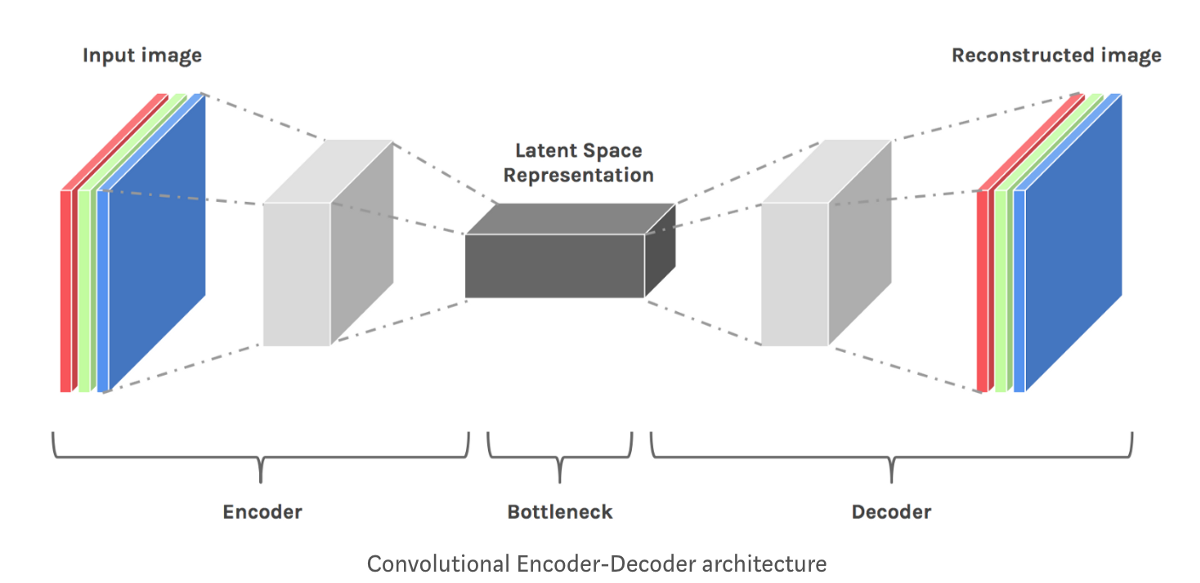
\includegraphics[width=12cm, height=5.2cm]{figs/AE_Arch.png}
    \caption{\href{https://hackernoon.com/latent-space-visualization-deep-learning-bits-2-bd09a46920df}{Source}}
    \end{figure}
}

%%%%%%%%%%%%%%%%%%%%%%%%%%%%%%%%%%%%%%%%%%%%%%%%%%%%%%%%%%%%%%%%%%%%%%%%%%%%%%%%%%%%%%%%%%%%%%%
\section{Denoising AE}
%%%%%%%%%%%%%%%%%%%%%%%%%%%%%%%%%%%%%%%%%%%%%%%%%%%%%%%%%%%%%%%%%%%%%%%%%%%%%%%%%%%%%%%%%%%%%%%

\frame{\frametitle{Denoising Autoencoders (DAE)}

\begin{itemize}	
    \normalsize{
    \item An AE learns the identity function which brings the risk of\tc{keywords}{overfitting}
    \item A DAE forces the model to learn a\tc{keywords}{more robust}latent representation
    \item It can also be used to efficiently\tc{keywords}{remove noise}from noisy images
    }
\end{itemize}


\begin{figure}
    \captionsetup{justification=centering, margin=1cm}
    % \vspace{-0.3cm}
    \centering
    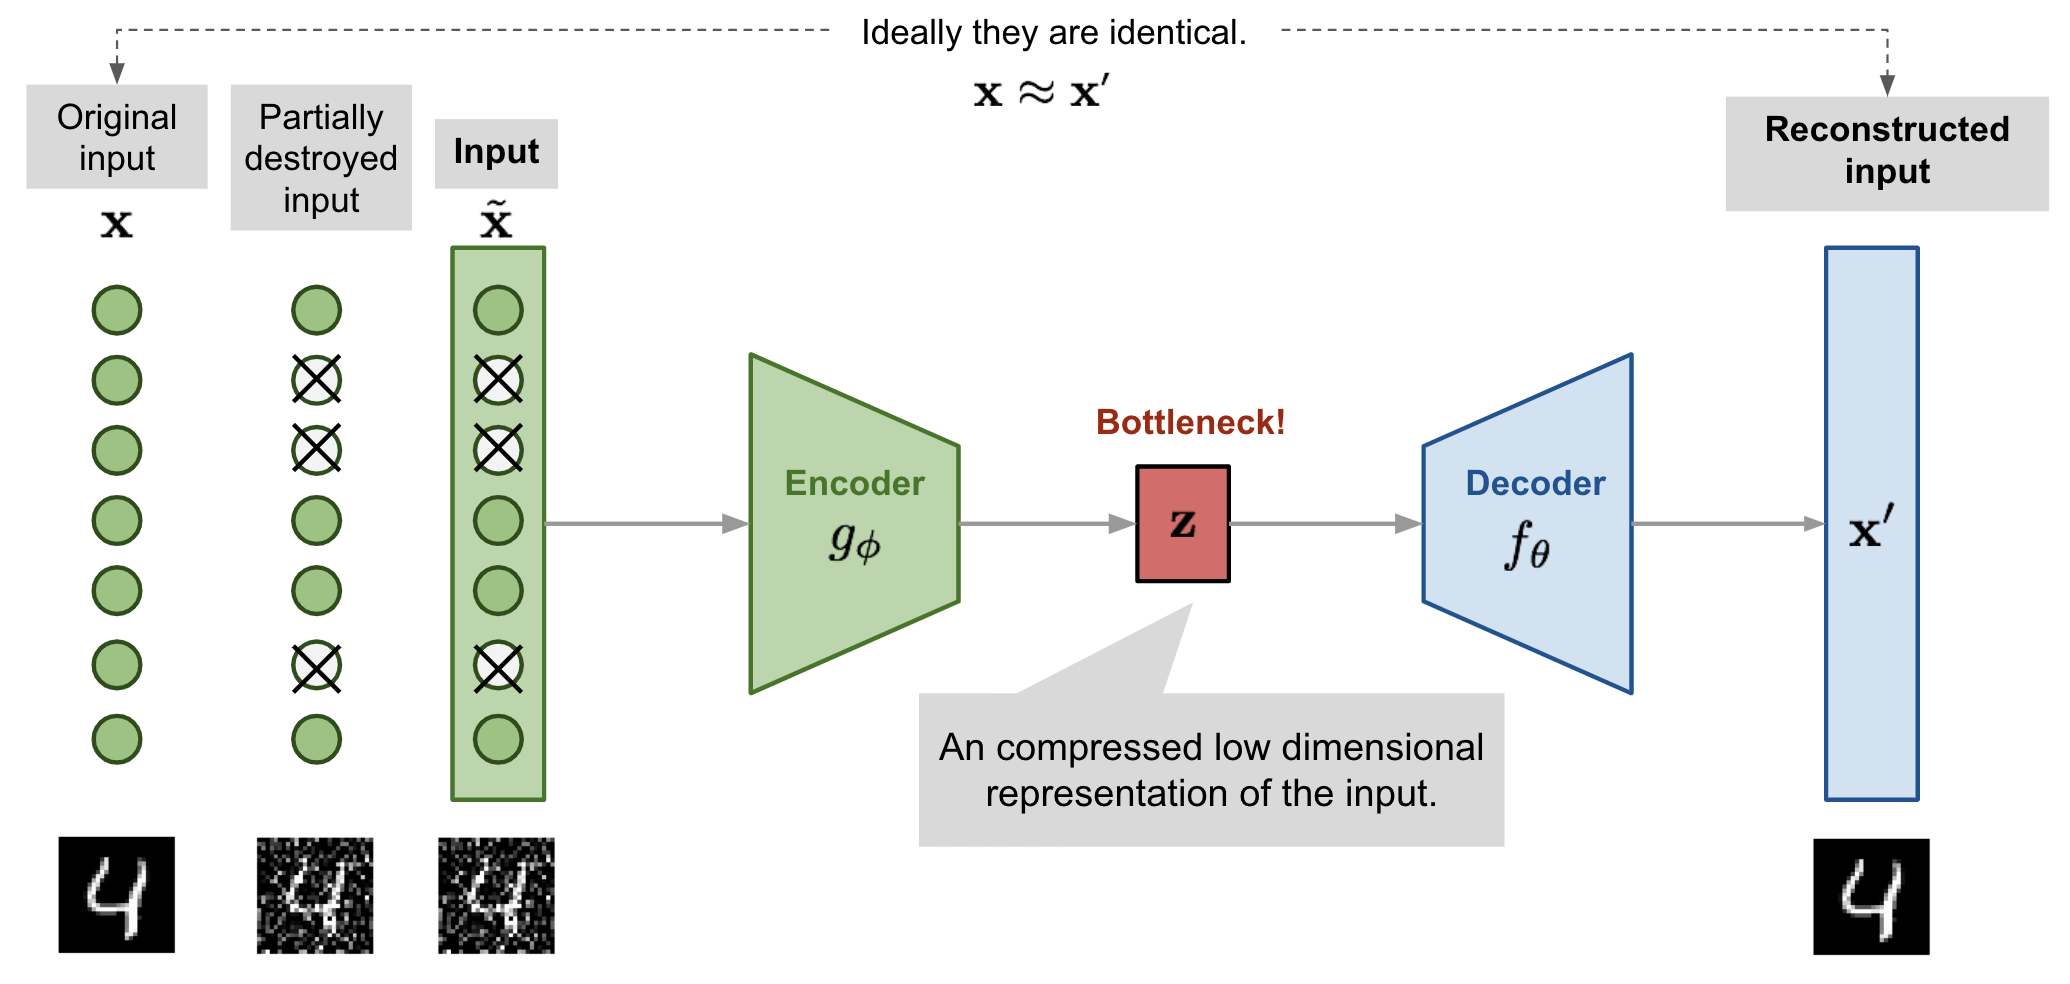
\includegraphics[width=12cm, height=5.2cm]{figs/denoising-autoencoder-architecture.png}
    \caption{Illustration of denoising autoencoder model architecture, \href{https://lilianweng.github.io/posts/2018-08-12-vae/}{Source}}
\end{figure}
}

%%%%%%%%%%%%%%%%%%%%%%%%%%%%%%%%%%%%%%%%%%%%%%%%%%%%%%%%%%%%%%%%%%%%%%%%%%%%%%%%%%%%%%%%%%%%%%%

\frame{\frametitle{Denoising Autoencoders}

\begin{itemize}	
    \item \normalsize Results of an autoencoder, predicting what the original data was, without even seeing it
\end{itemize}
\begin{figure}
    \centering
    \captionsetup{justification=centering, margin=1cm, labelformat=empty}
    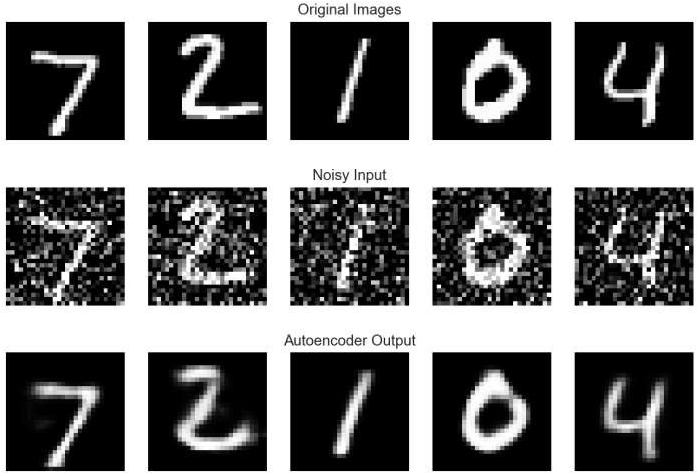
\includegraphics[width=12cm, height=5cm]{figs/noise_reduction.png}
    \caption{\href{https://towardsdatascience.com/applied-deep-learning-part-3-autoencoders-1c083af4d798}{Source}}
\end{figure}


}

%%%%%%%%%%%%%%%%%%%%%%%%%%%%%%%%%%%%%%%%%%%%%%%%%%%%%%%%%%%%%%%%%%%%%%%%%%%%%%%%%%%%%%%%%%%%%%%

\frame{\frametitle{Denoising Autoencoders}

\begin{itemize}	
    \normalsize{
    \item 
    DAEs won't simply memorize the inputs and outputs (More robustness)
    
    \item
    Intuitively, a DAE learns a\tc{keywords}{projection}from a neighborhood of our training data back onto the training data (\href{https://www.math.purdue.edu/~buzzard/MA598-Spring2019/Lectures/Lec16\%20-\%20Autoencoders.pptx}{Refrence})
    }
\end{itemize}

\begin{figure}
    \centering
    \captionsetup{justification=centering, margin=1cm, labelformat=empty}
    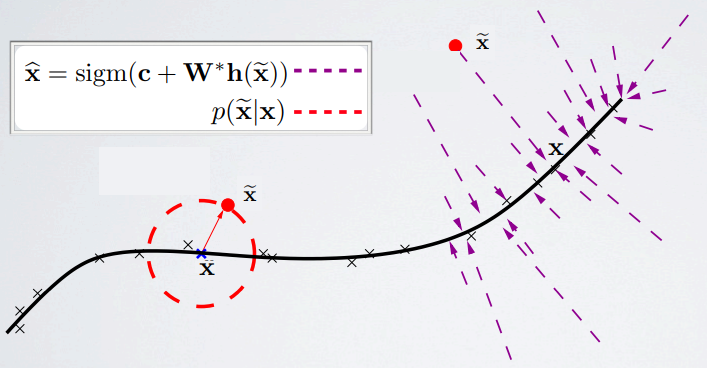
\includegraphics[width=12cm, height=5cm]{figs/denoise-theory1.png}
    \caption{\href{https://info.usherbrooke.ca/hlarochelle/ift725/6_06_denoising_autoencoder.pdf}{Source}}
\end{figure}
}

%%%%%%%%%%%%%%%%%%%%%%%%%%%%%%%%%%%%%%%%%%%%%%%%%%%%%%%%%%%%%%%%%%%%%%%%%%%%%%%%%%%%%%%%%%%%%%%

\frame{\frametitle{Denoising Autoencoders}

\begin{itemize}	
    \normalsize{
    \item 
    DAEs won't simply memorize the inputs and outputs (More robustness)
    
    \item
    Intuitively, a DAE learns a\tc{keywords}{projection}from a neighborhood of our training data back onto the training data (\href{https://www.math.purdue.edu/~buzzard/MA598-Spring2019/Lectures/Lec16\%20-\%20Autoencoders.pptx}{Refrence})
    }
\end{itemize}

\begin{figure}
    \centering
    \captionsetup{justification=centering, margin=1cm, labelformat=empty}
    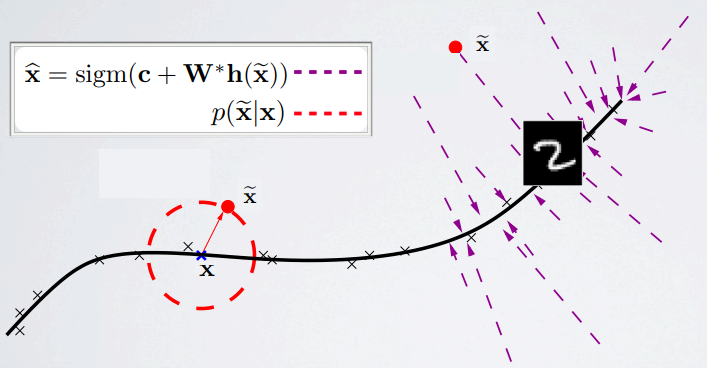
\includegraphics[width=12cm, height=5cm]{figs/denoise-theory2.png}
    \caption{\href{https://info.usherbrooke.ca/hlarochelle/ift725/6_06_denoising_autoencoder.pdf}{Source}}
\end{figure}
}
%%%%%%%%%%%%%%%%%%%%%%%%%%%%%%%%%%%%%%%%%%%%%%%%%%%%%%%%%%%%%%%%%%%%%%%%%%%%%%%%%%%%%%%%%%%%%%%

\frame{\frametitle{Denoising Autoencoders}

\begin{itemize}	
    \normalsize{
    \item 
    DAEs won't simply memorize the inputs and outputs (More robustness)
    
    \item
    Intuitively, a DAE learns a\tc{keywords}{projection}from a neighborhood of our training data back onto the training data (\href{https://www.math.purdue.edu/~buzzard/MA598-Spring2019/Lectures/Lec16\%20-\%20Autoencoders.pptx}{Refrence})
    }
\end{itemize}

\begin{figure}
    \centering
    \captionsetup{justification=centering, margin=1cm, labelformat=empty}
    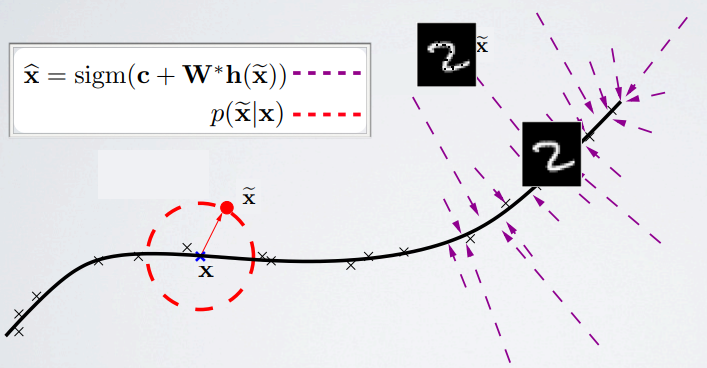
\includegraphics[width=12cm, height=5cm]{figs/denoise-theory3.png}
    \caption{\href{https://info.usherbrooke.ca/hlarochelle/ift725/6_06_denoising_autoencoder.pdf}{Source}}
\end{figure}
}
%%%%%%%%%%%%%%%%%%%%%%%%%%%%%%%%%%%%%%%%%%%%%%%%%%%%%%%%%%%%%%%%%%%%%%%%%%%%%%%%%%%%%%%%%%%%%%%

\frame{\frametitle{Denoising Autoencoders}

\begin{itemize}	
    \normalsize{
    \item 
    DAEs won't simply memorize the inputs and outputs (More robustness)
    
    \item
    Intuitively, a DAE learns a\tc{keywords}{projection}from a neighborhood of our training data back onto the training data (\href{https://www.math.purdue.edu/~buzzard/MA598-Spring2019/Lectures/Lec16\%20-\%20Autoencoders.pptx}{Refrence})
    }
\end{itemize}

\begin{figure}
    \centering
    \captionsetup{justification=centering, margin=1cm, labelformat=empty}
    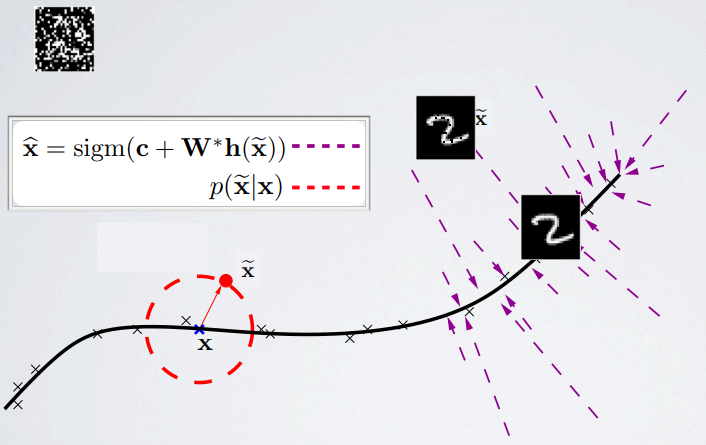
\includegraphics[width=12cm, height=5cm]{figs/denoise-theory4.png}
    \caption{\href{https://info.usherbrooke.ca/hlarochelle/ift725/6_06_denoising_autoencoder.pdf}{Source}}
\end{figure}
}
%%%%%%%%%%%%%%%%%%%%%%%%%%%%%%%%%%%%%%%%%%%%%%%%%%%%%%%%%%%%%%%%%%%%%%%%%%%%%%%%%%%%%%%%%%%%%%%
\section{Variaional AE}
%%%%%%%%%%%%%%%%%%%%%%%%%%%%%%%%%%%%%%%%%%%%%%%%%%%%%%%%%%%%%%%%%%%%%%%%%%%%%%%%%%%%%%%%%%%%%%%
\frame{\frametitle{Autoencoder Generative Models}

	
	\centering
    % \vspace{25 pt}
    \textbf{\large{How can we generate {\color{hotpink}{NEW}} data with Autoencoders??}}
    \vspace{5 pt}
    \newline
    hint: Autoencoder learns the feature space!

    

}

%%%%%%%%%%%%%%%%%%%%%%%%%%%%%%%%%%%%%%%%%%%%%%%%%%%%%%%%%%%%%%%%%%%%%%%%%%%%%%%%%%%%%%%%%%%%%%%

\frame{\frametitle{Walking through an example}

\begin{itemize}	
    \normalsize{
    \item 
    We can try to decode a\tc{keywords}{random point}from the latent space to generate new data
    \item
    The freedom of AEs leads to a severe overfitting which results in some points of the latent space being\tc{keywords}{meaningless}once decoded
    }
\end{itemize}
\vspace{-0.4cm}
\begin{figure}
    \centering
    \captionsetup{justification=centering, margin=1cm}
    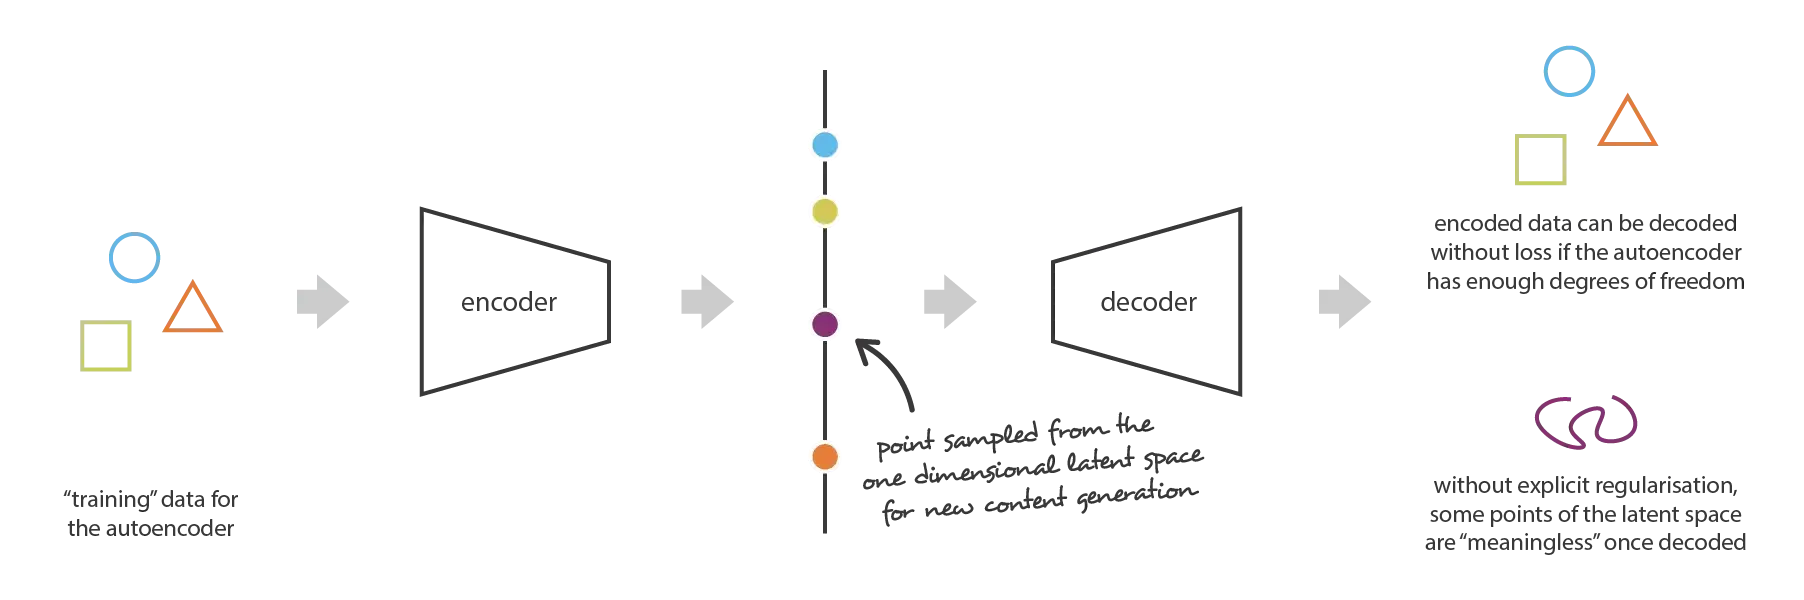
\includegraphics[width=12cm, height=5cm]{figs/vae1.png}
    \caption{Irregular latent space prevent us from using autoencoder for new content generation, \href{https://towardsdatascience.com/understanding-variational-autoencoders-vaes-f70510919f73}{Source}}
\end{figure}
}

%%%%%%%%%%%%%%%%%%%%%%%%%%%%%%%%%%%%%%%%%%%%%%%%%%%%%%%%%%%%%%%%%%%%%%%%%%%%%%%%%%%%%%%%%%%%%%%

\frame{\frametitle{Walking through an example}

\begin{itemize}	
    \item \normalsize Not all of the points in latent space have meaningful reconstructions
\end{itemize}


\begin{figure}
    \centering
    \vspace{-0.5cm}
    \captionsetup{justification=centering, margin=1cm}
    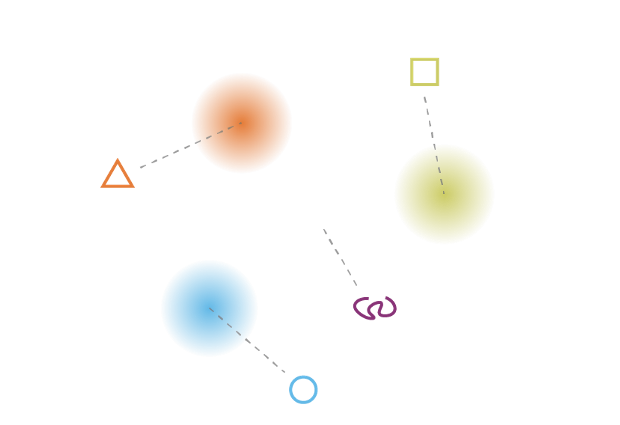
\includegraphics[width=9cm]{figs/vae_2_1.png}
    \caption{Latent space and the decoded outputs for some points in it, \href{https://towardsdatascience.com/understanding-variational-autoencoders-vaes-f70510919f73}{Source}}
\end{figure}
}

%%%%%%%%%%%%%%%%%%%%%%%%%%%%%%%%%%%%%%%%%%%%%%%%%%%%%%%%%%%%%%%%%%%%%%%%%%%%%%%%%%%%%%%%%%%%%%%

\frame{\frametitle{Walking through an example}

\begin{itemize}	
    \item \normalsize
    What we want is something like the following picture. So that with sampling from the latent space, we can generate new shapes.

\end{itemize}

\begin{figure}
    \centering
    \captionsetup{justification=centering, margin=1cm}
    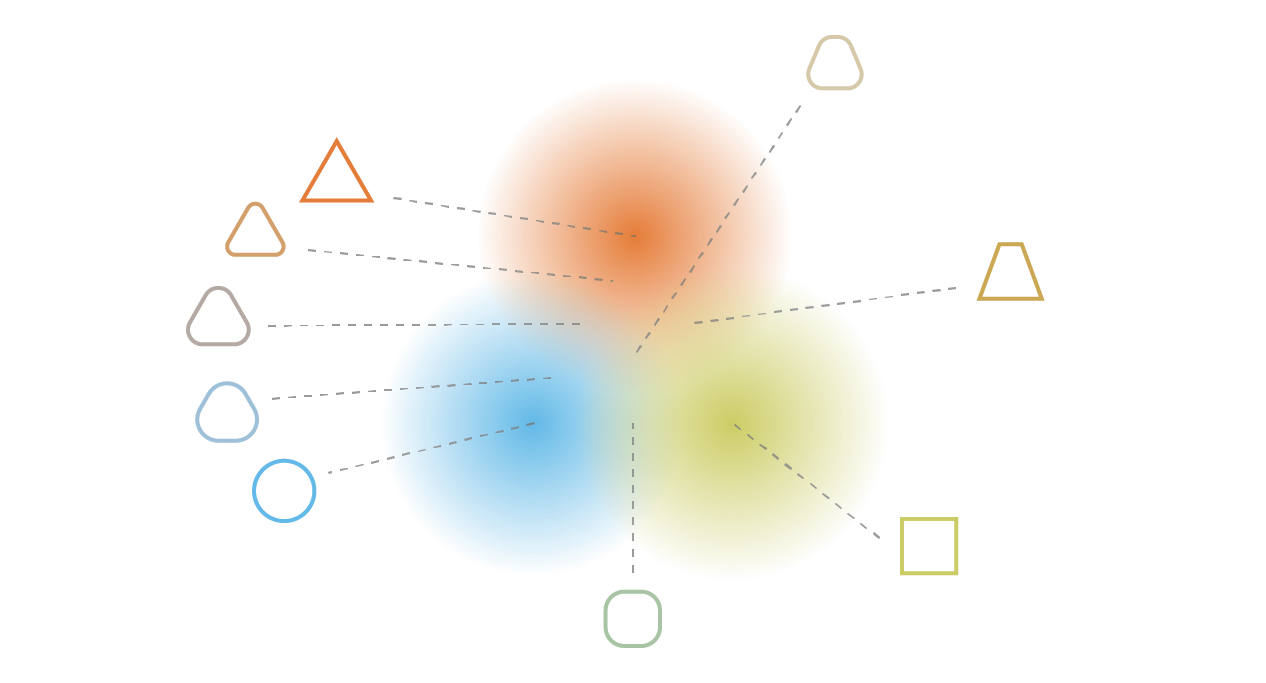
\includegraphics[width=9cm]{figs/vae_3.png}
    \caption{Regularisation tends to create a “gradient” over the information encoded in the latent space, \href{https://towardsdatascience.com/understanding-variational-autoencoders-vaes-f70510919f73}{Source}}
\end{figure}
}

%%%%%%%%%%%%%%%%%%%%%%%%%%%%%%%%%%%%%%%%%%%%%%%%%%%%%%%%%%%%%%%%%%%%%%%%%%%%%%%%%%%%%%%%%%%%%%%

\frame{\frametitle{Variational Autoencoders}
	\centering
    \textbf{\large{Ideas for solving this problem?}}
}

%%%%%%%%%%%%%%%%%%%%%%%%%%%%%%%%%%%%%%%%%%%%%%%%%%%%%%%%%%%%%%%%%%%%%%%%%%%%%%%%%%%%%%%%%%%%%%%

\frame{\frametitle{Variational Autoencoders}
\centering
\vspace{-0.3cm}
\begin{itemize}
    \normalsize{
    \item Instead of encoding the input into a single point (the latent representation), we encode it into a distribution over the latent space
    \item Then we can sample our latent representation from the latent distribution
    }
\end{itemize}

\begin{figure}
    \centering
    \vspace{-0.8cm}
    \captionsetup{justification=centering, margin=1cm}
    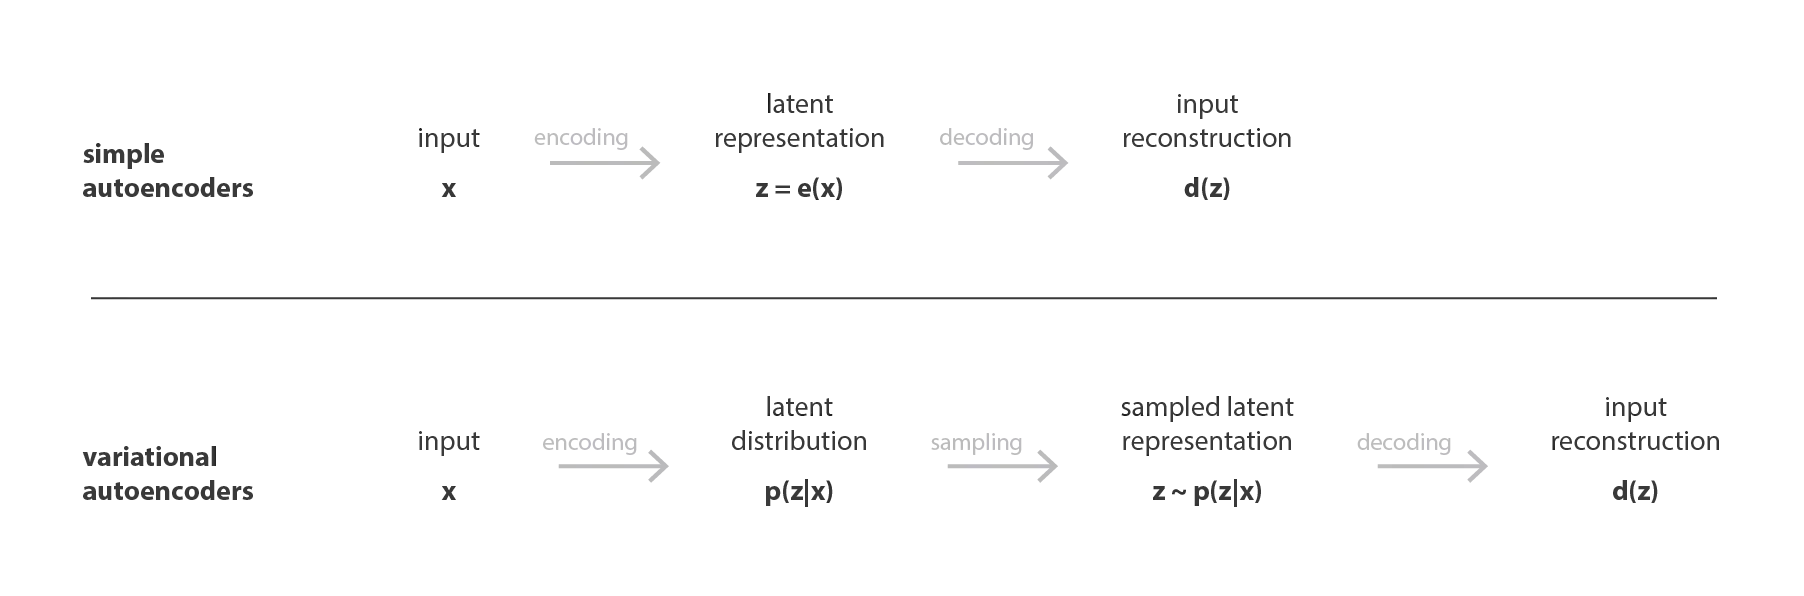
\includegraphics[width=12cm, height=5cm]{figs/vae4.png}
    \caption{Difference between autoencoder (deterministic) and variational autoencoder (probabilistic), \href{https://towardsdatascience.com/understanding-variational-autoencoders-vaes-f70510919f73}{Source}}
\end{figure}
}

%%%%%%%%%%%%%%%%%%%%%%%%%%%%%%%%%%%%%%%%%%%%%%%%%%%%%%%%%%%%%%%%%%%%%%%%%%%%%%%%%%%%%%%%%%%%%%%

\frame{\frametitle{Variational Autoencoders}
\centering
% \vspace{-0.3cm}
\begin{itemize}
    \normalsize{
    \item We will be encoding into, and sampling from normal distributions
    \item So our encoder needs to return the mean and the variance matrix, describing these Gaussians
    }
\end{itemize}

\begin{figure}
    \centering
    % \vspace{-0.5cm}
    \captionsetup{justification=centering}
    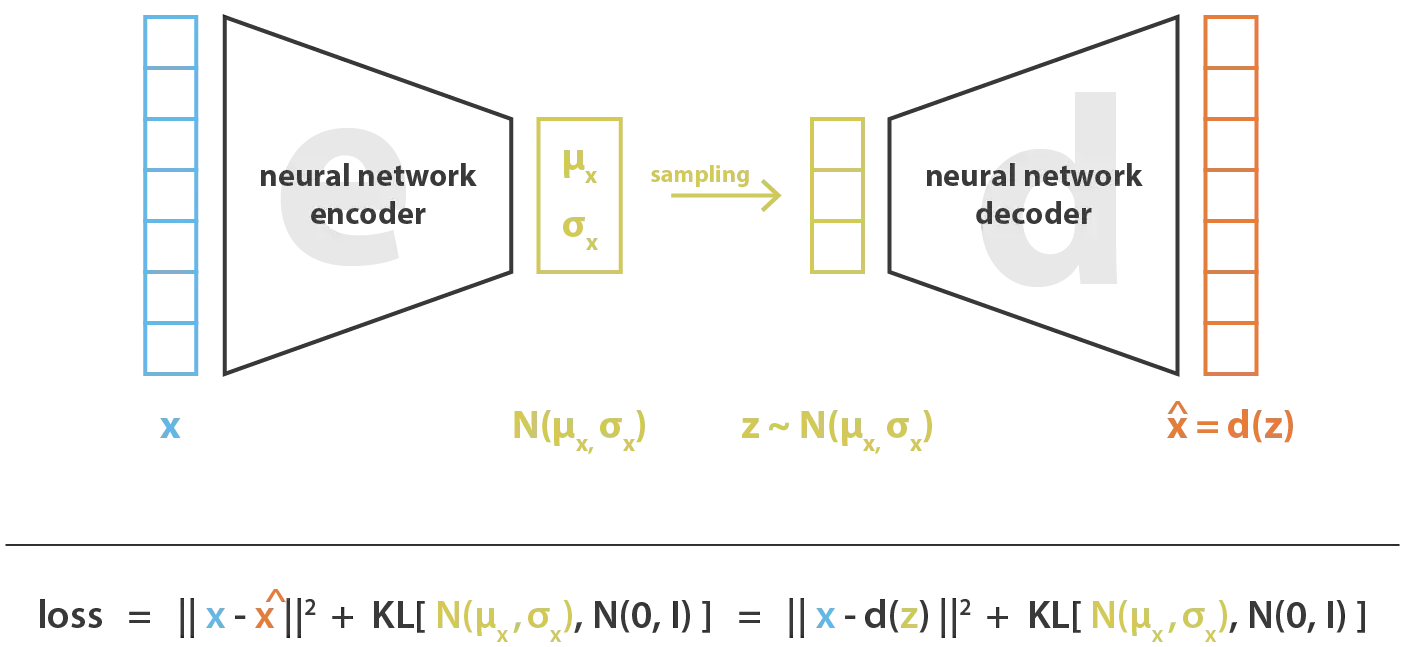
\includegraphics[width=10.7cm]{figs/vae6.png}
    \caption{In variational autoencoders, the loss function is composed of a reconstruction term (that makes the encoding-decoding scheme efficient) and a regularization term (that makes the latent space regular), \href{https://towardsdatascience.com/understanding-variational-autoencoders-vaes-f70510919f73}{Source}}
\end{figure}
}

%%%%%%%%%%%%%%%%%%%%%%%%%%%%%%%%%%%%%%%%%%%%%%%%%%%%%%%%%%%%%%%%%%%%%%%%%%%%%%%%%%%%%%%%%%%%%%%

\frame{\frametitle{Variational Autoencoders}
\centering
% \vspace{-0.3cm}
\begin{itemize}
    \normalsize{
    \item Encoding as distributions, will make it possible to express a good latent space regularization:
        \begin{itemize}
            \item {The distribution returned will be forced to be close to the standard normal distribution (Mean=0, Var=1) {\rightarrow} \(\mathcal{N}(0,\,1)\)}
        \end{itemize}
    }
\end{itemize}

\begin{figure}
    \centering
    % \vspace{-0.5cm}
    \captionsetup{justification=centering}
    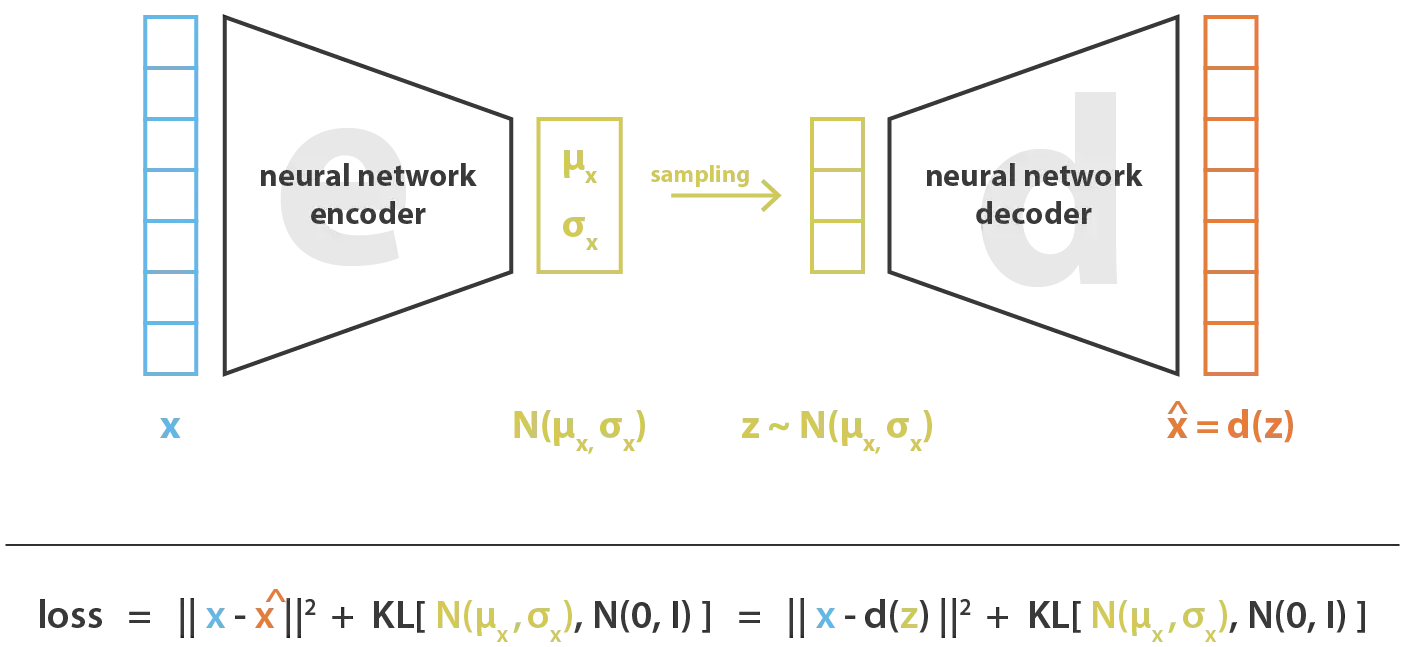
\includegraphics[width=10cm]{figs/vae6.png}
    \caption{In variational autoencoders, the loss function is composed of a reconstruction term (that makes the encoding-decoding scheme efficient) and a regularisation term (that makes the latent space regular), \href{https://towardsdatascience.com/understanding-variational-autoencoders-vaes-f70510919f73}{Source}}
\end{figure}
}

%%%%%%%%%%%%%%%%%%%%%%%%%%%%%%%%%%%%%%%%%%%%%%%%%%%%%%%%%%%%%%%%%%%%%%%%%%%%%%%%%%%%%%%%%%%%%%%

\frame{\frametitle{Variational Autoencoders}
\centering
% \vspace{-0.3cm}
\begin{itemize}
    \normalsize{
    \item The regularization term is expressed as the Kulback-Leibler divergence between the returned distribution and a standard Gaussian:
    \vspace{0.1cm}
    \begin{itemize}
        \item \(KL(\mathcal{N}(\mu_x,\,\sigma_x) || \mathcal{N}(0,\,1))\)
    \end{itemize}
    }
\end{itemize}

\begin{figure}
    \centering
    % \vspace{-0.5cm}
    \captionsetup{justification=centering}
    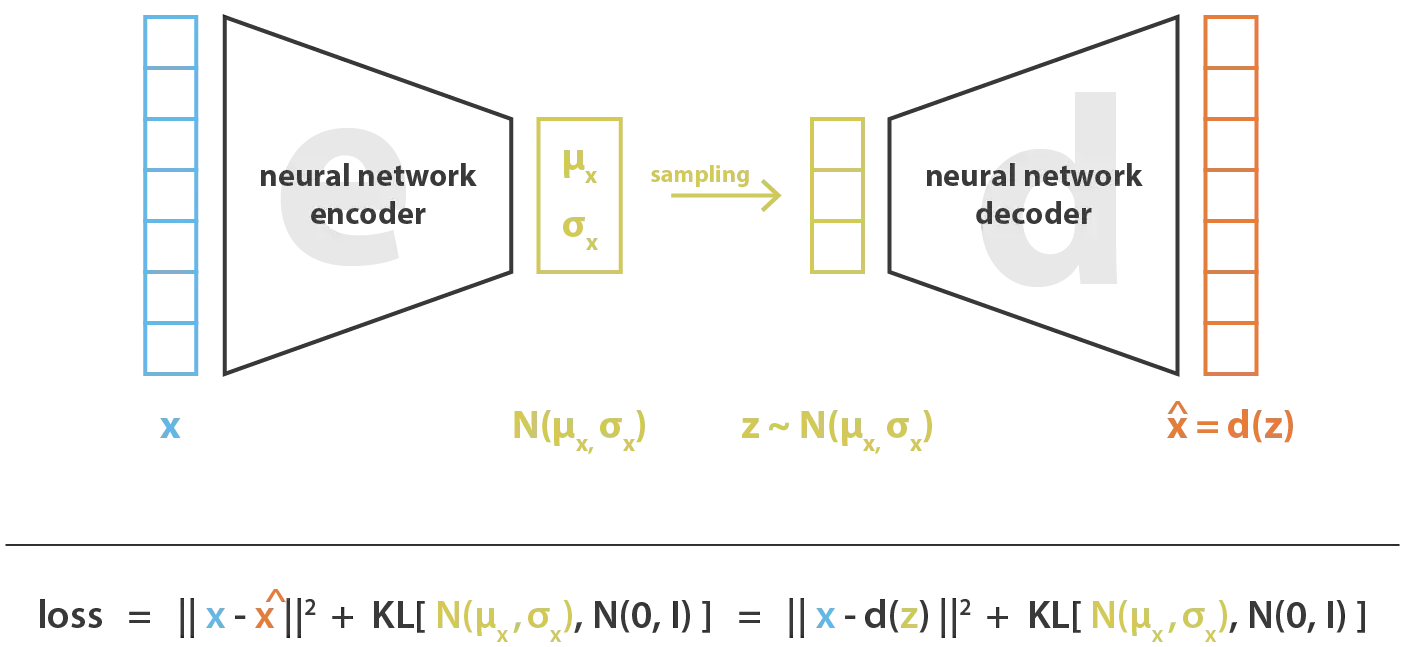
\includegraphics[width=10.6cm]{figs/vae6.png}
    \caption{In variational autoencoders, the loss function is composed of a reconstruction term (that makes the encoding-decoding scheme efficient) and a regularisation term (that makes the latent space regular), \href{https://towardsdatascience.com/understanding-variational-autoencoders-vaes-f70510919f73}{Source}}
\end{figure}
}

%%%%%%%%%%%%%%%%%%%%%%%%%%%%%%%%%%%%%%%%%%%%%%%%%%%%%%%%%%%%%%%%%%%%%%%%%%%%%%%%%%%%%%%%%%%%%%%

\frame{\frametitle{Effect of regularization}
\centering
% \vspace{-0.3cm}
\begin{itemize}
    \normalsize{
    \item This regularity brings two main properties:
    \vspace{0.1cm}
    \begin{itemize}
        \item \tc{keywords}{Continuity}: Two close points in the latent space should not give two completely different contents once decoded
        \item \tc{keywords}{Completeness}: For a chosen distribution, a point sampled from the latent space should give “meaningful” content once decoded
    \end{itemize}
    }
\end{itemize}

\begin{figure}
    \centering
    % \vspace{-0.5cm}
    \captionsetup{justification=centering}
    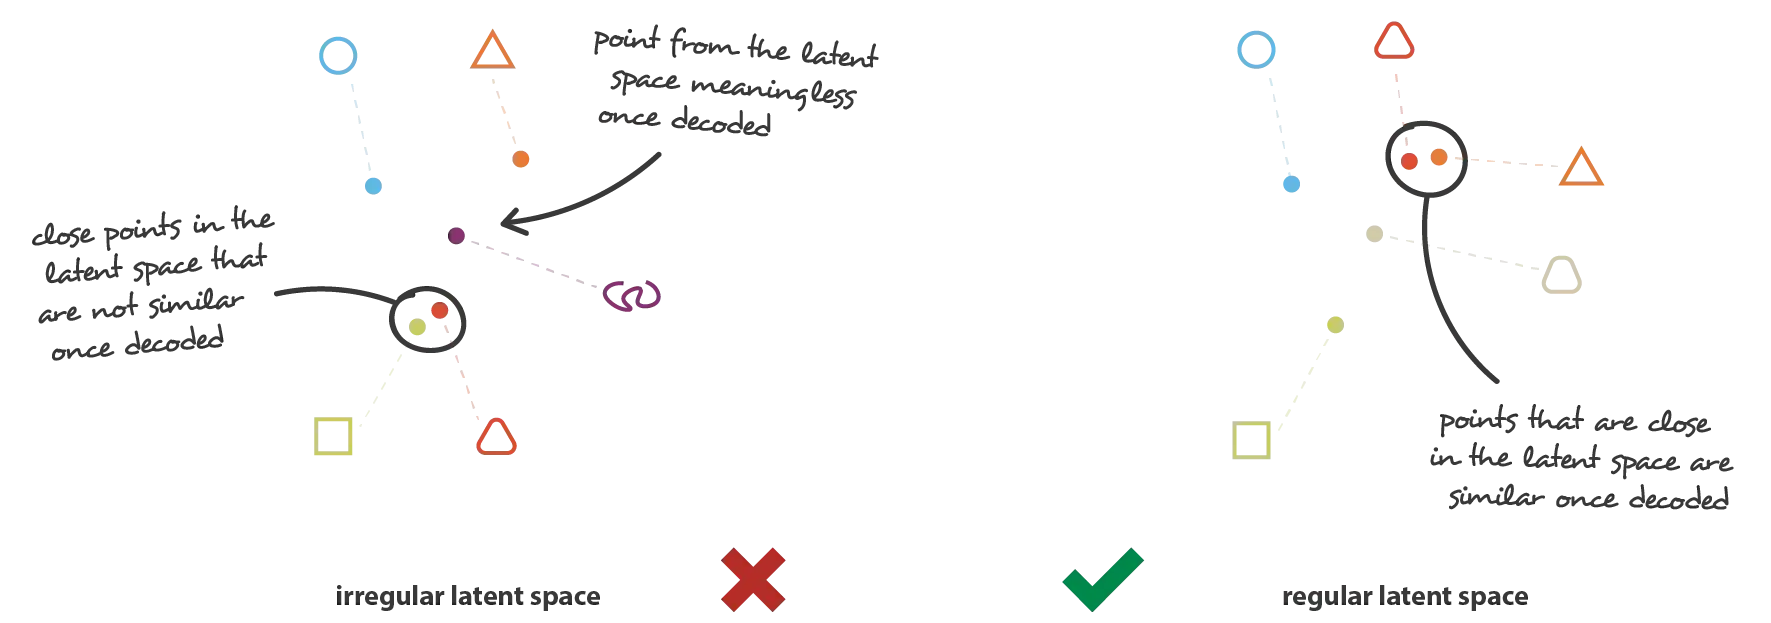
\includegraphics[width=12cm]{figs/vae7.png}
    \caption{Difference between a “regular” and an “irregular” latent space, \href{https://towardsdatascience.com/understanding-variational-autoencoders-vaes-f70510919f73}{Source}}
\end{figure}
}

%%%%%%%%%%%%%%%%%%%%%%%%%%%%%%%%%%%%%%%%%%%%%%%%%%%%%%%%%%%%%%%%%%%%%%%%%%%%%%%%%%%%%%%%%%%%%%%

\frame{\frametitle{In practice}
\centering
% \vspace{-0.3cm}
\begin{itemize}
    \normalsize{
    \item We will use two networks at the end of our encoder to calculate the mean and variance
    }
\end{itemize}
\normalsize{\centering {$g(x) = g_2(g_1(x)) \qquad h(x) = h_2(h_1(x)) \qquad g_1(x)=h_1(x)$}}

\begin{figure}
    \centering
    % \vspace{-0.5cm}
    \captionsetup{justification=centering}
    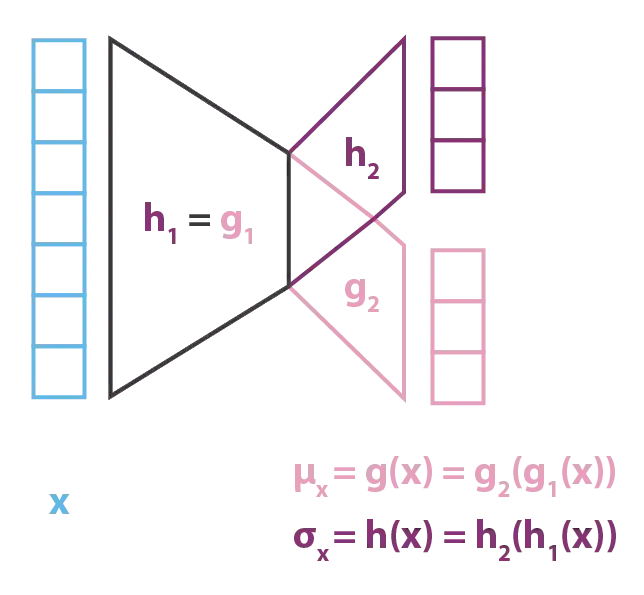
\includegraphics[width=5.5cm]{figs/vae8.png}
    \caption{Encoder part of the VAE, \href{https://towardsdatascience.com/understanding-variational-autoencoders-vaes-f70510919f73}{Source}}
\end{figure}
}

%%%%%%%%%%%%%%%%%%%%%%%%%%%%%%%%%%%%%%%%%%%%%%%%%%%%%%%%%%%%%%%%%%%%%%%%%%%%%%%%%%%%%%%%%%%%%%%

\frame{\frametitle{Reparameterization Trick}
\centering
\vspace{-0.7cm}
\begin{itemize}
    \normalsize{
    \item Problem: We cannot perform\tc{keywords}{backpropagation}on the direct sampling operation
    }
\end{itemize}

\begin{figure}
    \centering
    % \vspace{-0.5cm}
    \captionsetup{justification=centering}
    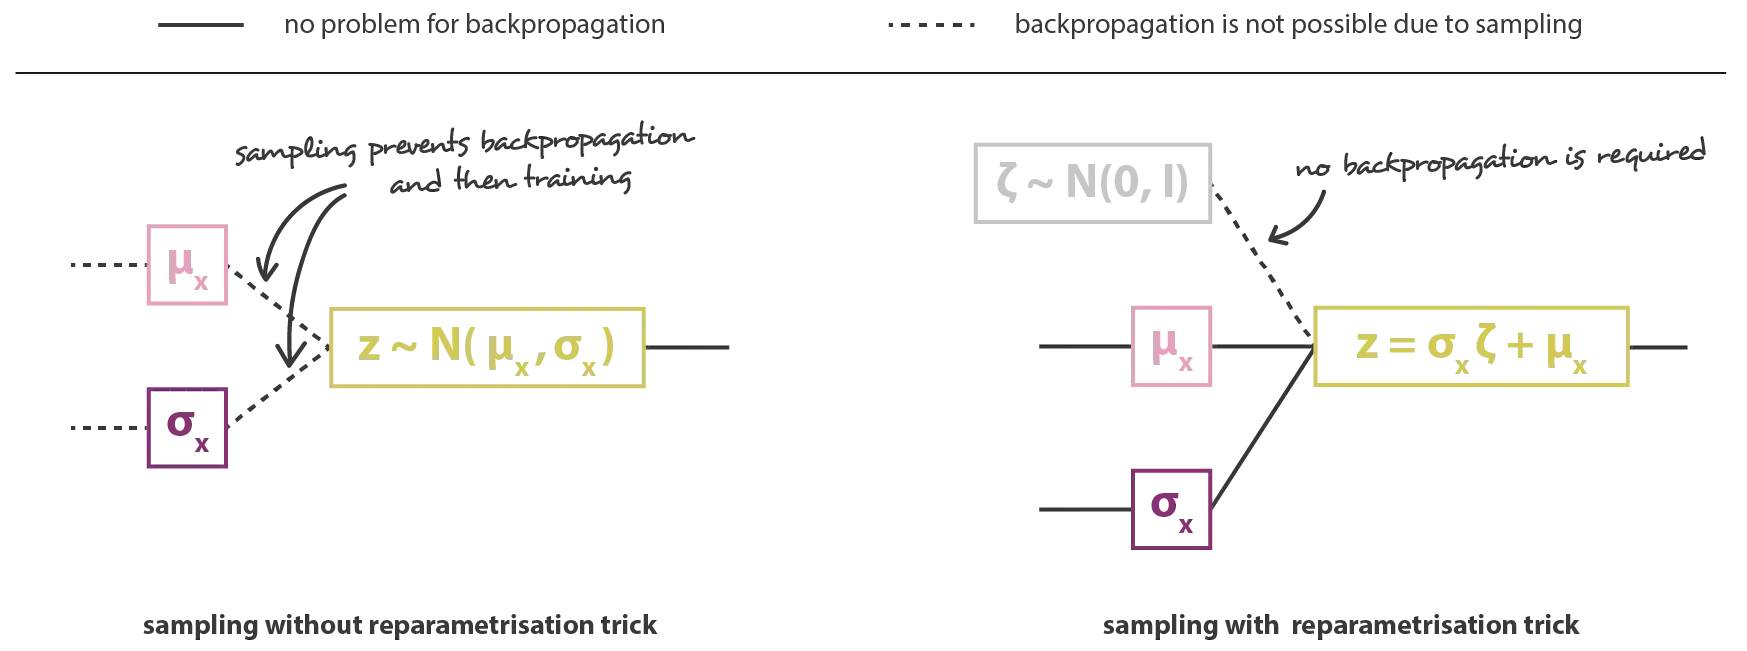
\includegraphics[width=12cm]{figs/vae9.png}
    \caption{Illustration of the reparameterization trick, \href{https://towardsdatascience.com/understanding-variational-autoencoders-vaes-f70510919f73}{Source}}
\end{figure}
}

%%%%%%%%%%%%%%%%%%%%%%%%%%%%%%%%%%%%%%%%%%%%%%%%%%%%%%%%%%%%%%%%%%%%%%%%%%%%%%%%%%%%%%%%%%%%%%%

\frame{\frametitle{Reparameterization Trick}
\centering
\vspace{-0.5cm}
\begin{itemize}
    \normalsize{
    \item Solution:\tc{keywords}{Reparameterization trick}
    \begin{itemize}
        \item We sample from a standard normal distribution and do the following operations to be able to track gradients
    \end{itemize}
    }
\end{itemize}
\begin{figure}
    \centering
    % \vspace{-0.5cm}
    \captionsetup{justification=centering}
    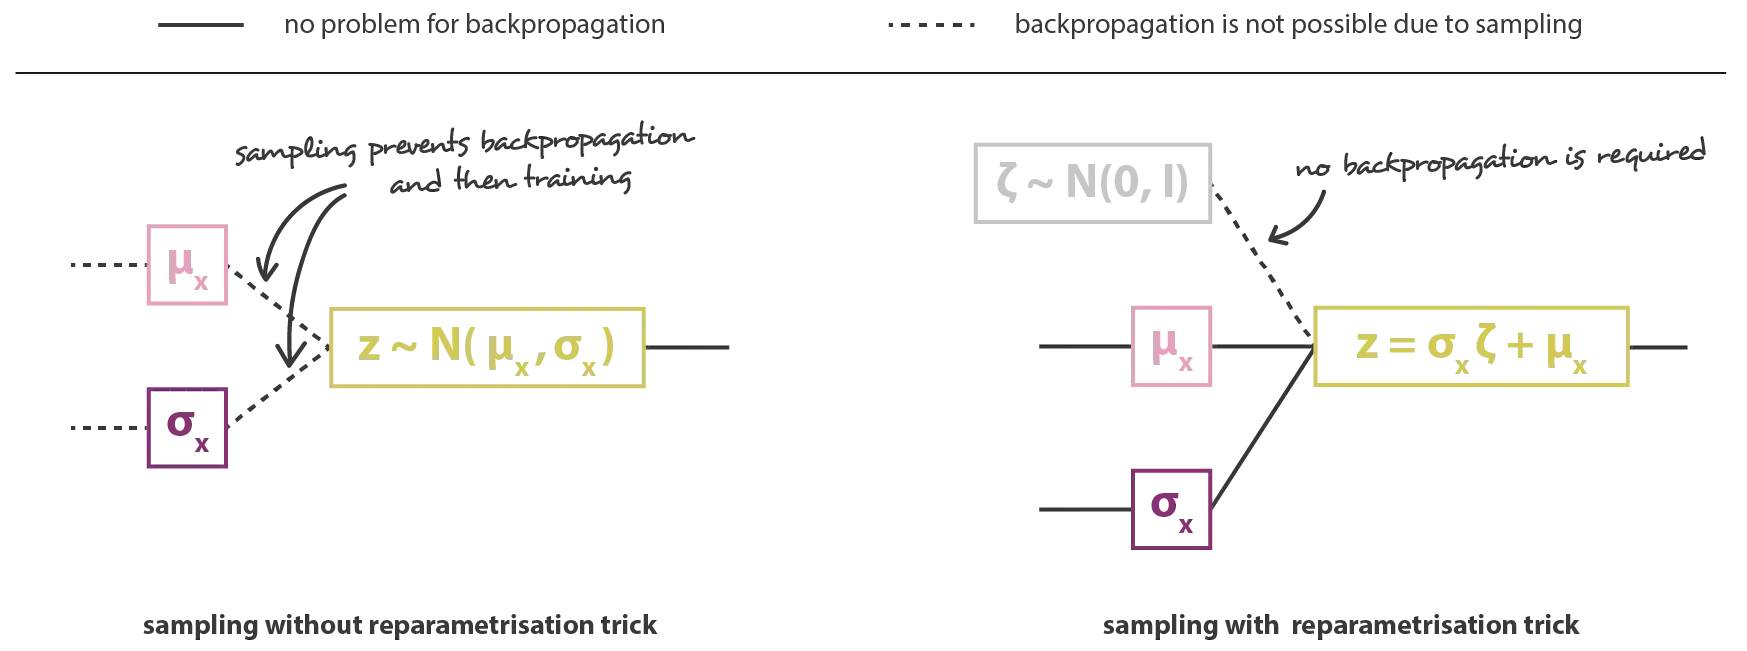
\includegraphics[width=12cm]{figs/vae9.png}
    \caption{Illustration of the reparameterization trick, \href{https://towardsdatascience.com/understanding-variational-autoencoders-vaes-f70510919f73}{Source}}
\end{figure}
}
%%%%%%%%%%%%%%%%%%%%%%%%%%%%%%%%%%%%%%%%%%%%%%%%%%%%%%%%%%%%%%%%%%%%%%%%%%%%%%%%%%%%%%%%%%%%%%%

\frame{\frametitle{The Whole Picture}
\centering
% \vspace{-0.3cm}
\begin{itemize}
    \normalsize{
    \item The whole picture of a simple variational autoencoder:
    }
\end{itemize}

\begin{figure}
    \centering
    % \vspace{-0.5cm}
    \captionsetup{justification=centering}
    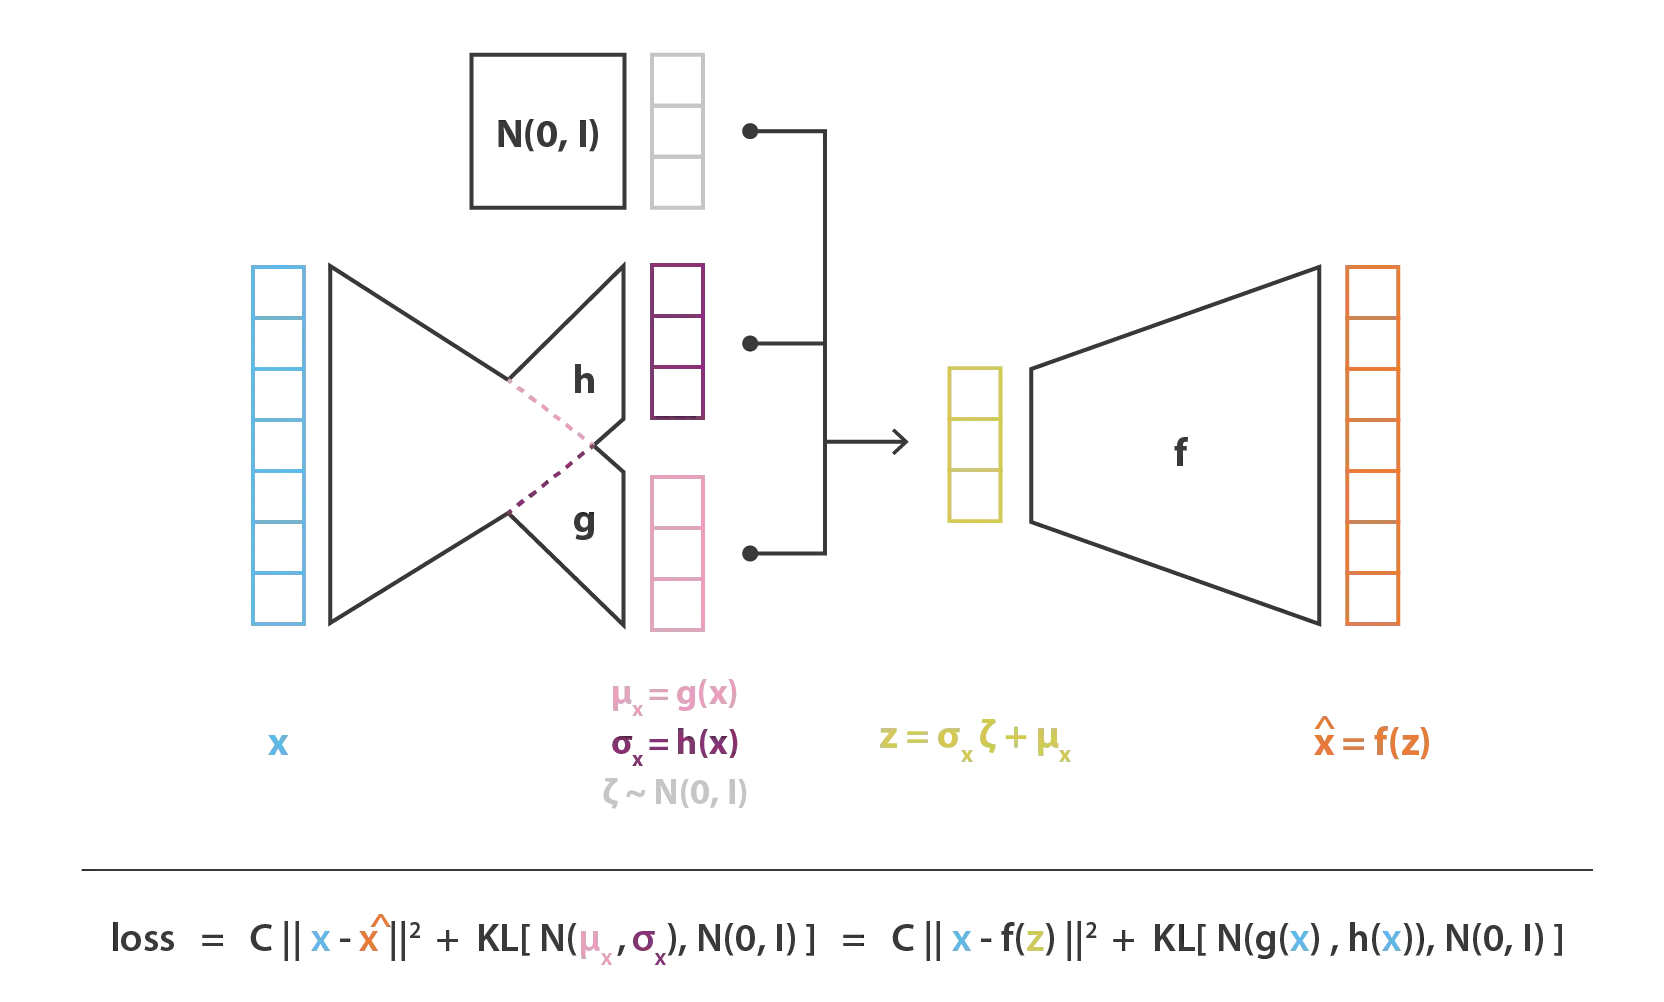
\includegraphics[width=12cm, height=6cm]{figs/vae11.png}
    \caption{Variational Autoencoders representation, \href{https://towardsdatascience.com/understanding-variational-autoencoders-vaes-f70510919f73}{Source}}
\end{figure}
}
%%%%%%%%%%%%%%%%%%%%%%%%%%%%%%%%%%%%%%%%%%%%%%%%%%%%%%%%%%%%%%%%%%%%%%%%%%%%%%%%%%%%%%%%%%%%%%%
\frame{\frametitle{Refrences}
\begin{itemize}
    \printbibliography
\end{itemize}
\bibliographystyle{plain}
\bibliography{Refrences}
}
%%%%%%%%%%%%%%%%%%%%%%%%%%%%%%%%%%%%%%%%%%%%%%%%%%%%%%%%%%%%%%%%%%%%%%%%%%%%%%%%%%%%%%%%%%%%%%%

\frametitle{Final Notes}
\centering
\vspace{50 pt}
\textbf{Thank You!}
\vspace{50pt}

\textbf{Any Question?}
%%%%%%%%%%%%%%%%%%%%%%%%%%%%%%%%%%%%%%%%%%
\end{document}